\documentclass{beamer}
\usefonttheme[onlymath]{serif}
%Information to be included in the title page:
\title{Elimination and cut-elimination in multiplicative linear logic}
\author{Daniel Murfet, William Troiani}
\institute{University of Melbourne, University of Sorbonne Paris Nord}
\date{2022}

\usepackage{amsthm}
\usepackage{amsmath}
\usepackage{amsfonts}
\usepackage{algorithm}
\usepackage{mathrsfs}
\usepackage{array}
\usepackage{amssymb}
\usepackage{units}
\usepackage{graphicx}
\usepackage{tikz-cd}
\usepackage{nicefrac}
\usepackage{hyperref}
\usepackage{bbm}
\usepackage{color}
\usepackage{tensor}
\usepackage{tipa}
\usepackage{bussproofs}
\usepackage{ stmaryrd }
\usepackage{ textcomp }
\usepackage{leftidx}
\usepackage{afterpage}
\usepackage{varwidth}
\usepackage{tasks}
\usepackage{ cmll }
\usepackage{makecell}
\usepackage{MnSymbol}
\usepackage{quiver}
\usepackage{adjustbox}
\usepackage{multirow}
\usepackage{booktabs}
\usepackage{xparse}
\usepackage{calc}

\newcommand\blankpage{
	\null
	\thispagestyle{empty}
	\addtocounter{page}{-1}
	\newpage
}

\graphicspath{ {images/} }

\theoremstyle{plain}
\newtheorem{thm}{Theorem}[subsection] % reset theorem numbering for each chapter
\newtheorem{proposition}[thm]{Proposition}
%\newtheorem{lemma}[thm]{Lemma}
%\newtheorem{fact}[thm]{Fact}
\newtheorem{cor}[thm]{Corollary}

\theoremstyle{definition}
\newtheorem{defn}[thm]{Definition} % definition numbers are dependent on theorem numbers
\newtheorem{exmp}[thm]{Example} % same for example numbers
\newtheorem{notation}[thm]{Notation}
\newtheorem{remark}[thm]{Remark}
\newtheorem{condition}[thm]{Condition}
\newtheorem{question}[thm]{Question}
\newtheorem{construction}[thm]{Construction}
\newtheorem{exercise}[thm]{Exercise}
%\newtheorem{example}[thm]{Example}
\newtheorem{aside}[thm]{Aside}

\def\doubleunderline#1{\underline{\underline{#1}}}
\newcommand{\bb}[1]{\mathbb{#1}}
\newcommand{\scr}[1]{\mathscr{#1}}
\newcommand{\call}[1]{\mathcal{#1}}
\newcommand{\psheaf}{\text{\underline{Set}}^{\scr{C}^{\text{op}}}}
\newcommand{\und}[1]{\underline{\hspace{#1 cm}}}
\newcommand{\adj}[1]{\text{\textopencorner}{#1}\text{\textcorner}}
\newcommand{\comment}[1]{}
\newcommand{\lto}{\longrightarrow}
\newcommand{\rone}{(\operatorname{R}\bold{1})}
\newcommand{\lone}{(\operatorname{L}\bold{1})}
\newcommand{\rimp}{(\operatorname{R} \multimap)}
\newcommand{\limp}{(\operatorname{L} \multimap)}
\newcommand{\rtensor}{(\operatorname{R}\otimes)}
\newcommand{\ltensor}{(\operatorname{L}\otimes)}
\newcommand{\rtrue}{(\operatorname{R}\top)}
\newcommand{\rwith}{(\operatorname{R}\\&)}
\newcommand{\lwithleft}{(\operatorname{L}\\&)_{\operatorname{left}}}
\newcommand{\lwithright}{(\operatorname{L}\\&)_{\operatorname{right}}}
\newcommand{\rplusleft}{(\operatorname{R}\oplus)_{\operatorname{left}}}
\newcommand{\rplusright}{(\operatorname{R}\oplus)_{\operatorname{right}}}
\newcommand{\lplus}{(\operatorname{L}\oplus)}
\newcommand{\prom}{(\operatorname{prom})}
\newcommand{\ctr}{(\operatorname{ctr})}
\newcommand{\der}{(\operatorname{der})}
\newcommand{\weak}{(\operatorname{weak})}
\newcommand{\exi}{(\operatorname{exists})}
\newcommand{\fa}{(\operatorname{for\text{ }all})}
\newcommand{\ex}{(\operatorname{ex})}
\newcommand{\cut}{(\operatorname{cut})}
\newcommand{\ax}{(\operatorname{ax})}
\newcommand{\negation}{\sim}
\newcommand{\true}{\top}
\newcommand{\false}{\bot}
\DeclareRobustCommand{\diamondtimes}{%
	\mathbin{\text{\rotatebox[origin=c]{45}{$\boxplus$}}}%
}
\newcommand{\tagarray}{\mbox{}\refstepcounter{equation}$(\theequation)$}
\newcommand{\startproof}[1]{
	\AxiomC{#1}
	\noLine
	\UnaryInfC{$\vdots$}
}
\newenvironment{scprooftree}[1]%
{\gdef\scalefactor{#1}\begin{center}\proofSkipAmount \leavevmode}%
	{\scalebox{\scalefactor}{\DisplayProof}\proofSkipAmount \end{center} }
\newcommand\Wider[2][3em]{%
	\makebox[\linewidth][c]{%
		\begin{minipage}{\dimexpr\textwidth+#1\relax}
			\raggedright#2
		\end{minipage}%
	}%
}
% https://tex.stackexchange.com/questions/63355/wrapping-cmidrule-in-a-macro
\ExplSyntaxOn
\makeatletter
\newcommand{\CMidRule}{\noalign\bgroup\@CMidRule{}}
\NewDocumentCommand{\@CMidRule}{
	m % Material to reinsert before cmidrule.
	O{0.0ex} % #1 = left adjust
	O{0.0ex} % #1 = right adjust
	m  %       #3 = columns to span
}{
	\peek_meaning_remove_ignore_spaces:NTF \CMidRule
	{ \@CMidRule { #1 \cmidrule[\cmidrulewidth](l{#2}r{#3}){#4} } }
	{ \egroup #1 \cmidrule[\cmidrulewidth](l{#2}r{#3}){#4} }
}
\makeatother
\ExplSyntaxOff

\newcommand{\PhantC}{\phantom{\colon}}%
\newcommand{\PhantSQ}{\phantom{\sqrt{\hspace{0.3ex}}}}

\newcommand\showdiv[1]{\overline{\smash{)}#1}}


\begin{document}
	
	\frame{\titlepage}
	
	\begin{frame}
		\frametitle{Geometry of Interaction}
			\begin{figure}
				\caption{Identification of variables in an intuitionsitic sequent calculus proof}
				\centering
				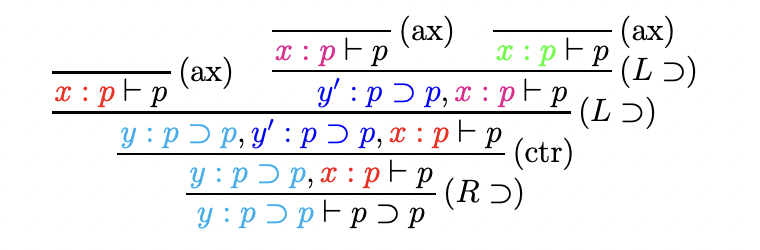
\includegraphics[width=0.75\textwidth]{PatternsOfEquality.png}
				\end{figure}
			Proof nets.
			\begin{center}
				\begin{tabular}{c c}
					$
					\begin{tikzcd}[column sep = small, row sep = small, ampersand replacement=\&]
						\& \ax\arrow[dl,bend right, dash]\arrow[dr,bend left, dash]\\
						\neg A\arrow[d] \& \& A\arrow[d]\\
						\vdots \& \& \vdots
					\end{tikzcd}$
					&
					$
					\begin{tikzcd}[column sep = small, row sep = small, ampersand replacement=\&]
						\vdots\arrow[d, dash] \& \& \vdots\arrow[d, dash]\\
						\neg A\arrow[dr,bend right] \& \& A\arrow[dl, bend left]\\
						\& \cut
					\end{tikzcd}$
				\end{tabular}
			\end{center}
	\end{frame}

\begin{frame}
	\[\adjustbox{scale=0.75}{\begin{tikzcd}[column sep = tiny, row sep = small, ampersand replacement=\&]
		\& \ax \&\&\&\& \ax \&\&\& \ax \\
		{\neg A_2} \&\& A_3 \&\& \neg A_{10} \&\& A_{11} \& \neg A_6 \&\& A_7 \\
		\, \&\&\& \otimes \&\&\& \, \&\& \parr \\
		\&\&\& A_4 \otimes \neg A_9 \&\&\&\&\& \neg A_5 \parr A_8 \\
		\&\&\&\&\&\& \cut
		\arrow[curve={height=12pt}, no head, from=1-2, to=2-1]
		\arrow[curve={height=-12pt}, no head, from=1-2, to=2-3]
		\arrow[from=2-1, to=3-1]
		\arrow[curve={height=12pt}, no head, from=1-6, to=2-5]
		\arrow[curve={height=-12pt}, no head, from=1-6, to=2-7]
		\arrow[from=2-7, to=3-7]
		\arrow[curve={height=-12pt}, from=2-5, to=3-4]
		\arrow[curve={height=12pt}, from=2-3, to=3-4]
		\arrow[curve={height=12pt}, no head, from=1-9, to=2-8]
		\arrow[curve={height=-12pt}, no head, from=1-9, to=2-10]
		\arrow[curve={height=-12pt}, from=2-10, to=3-9]
		\arrow[curve={height=12pt}, from=2-8, to=3-9]
		\arrow[no head, from=3-9, to=4-9]
		\arrow[curve={height=-12pt}, from=4-9, to=5-7]
		\arrow[curve={height=12pt}, from=4-4, to=5-7]
		\arrow[no head, from=3-4, to=4-4]
	\end{tikzcd}}\]
	\[\adjustbox{scale=0.75}{\begin{tikzcd}[column sep = tiny, row sep = small, ampersand replacement=\&]
		\&\&\&\&\& \ax \\
		\& \ax \&\&\& \neg A_{10} \&\& A_{11} \&\& \ax \\
		{\neg A_2} \&\& A_3 \&\&\&\& \, \& {\neg A_6} \&\& A_7 \\
		\&\&\&\& \cut \&\&\& \cut \\
		\,
		\arrow[curve={height=12pt}, no head, from=2-2, to=3-1]
		\arrow[curve={height=-12pt}, no head, from=2-2, to=3-3]
		\arrow[from=3-1, to=5-1]
		\arrow[curve={height=12pt}, no head, from=1-6, to=2-5]
		\arrow[curve={height=-12pt}, no head, from=1-6, to=2-7]
		\arrow[from=2-7, to=3-7]
		\arrow[curve={height=12pt}, no head, from=2-9, to=3-8]
		\arrow[curve={height=-12pt}, no head, from=2-9, to=3-10]
		\arrow[curve={height=12pt}, from=3-3, to=4-5]
		\arrow[curve={height=-12pt}, from=3-8, to=4-5]
		\arrow[curve={height=12pt}, from=2-5, to=4-8]
		\arrow[curve={height=-12pt}, from=3-10, to=4-8]
	\end{tikzcd}}\]
	\end{frame}

\begin{frame}
	The goals of this paper are to set up a basic dictionary between
	\begin{itemize}
		\item multiplicative proofs nets and ideals
		\item reduction sequences and monomial orders
		\item cut-elimination and elimination
	\end{itemize}
	The ideals $I_\pi$ do not have a very interesting geometry: the associated affine variety is just an intersection of pairwise diagonals. In subsequent papers in this series we introduce, on top of the foundations laid here, more interesting algebra and geometry (see Section 8).
	\end{frame}

\begin{frame}
	\frametitle{Formulas}
	\begin{defn}[Formulas]\label{def:formulas}
		\begin{itemize}
			\item \emph{Unoriented atoms} $X,Y,Z,...$
			\item \emph{An oriented atom} (or \emph{atomic proposition}) is a pair $(X,+)$ or $(X,-)$ where $X$ is an unoriented atom.
			\end{itemize}
	 \emph{Pre-formulas}:
	\begin{itemize}
		\item Any atomic proposition is a preformula.
		\item If $A,B$ are pre-formulas then so are $A \otimes B$, $A \parr B$.
		\item If $A$ is a pre-formula then so is $\neg A$.
	\end{itemize}
	\emph{Formulas}: quotient of pre-formulas:
	\begin{equation*}
		\neg (A \otimes B) \sim \neg B \parr \neg A \qquad \neg (A \parr B) \sim \neg B \otimes \neg A
		\end{equation*}
	\begin{equation*}
		\neg (X, +) \sim (X, -)\qquad \neg (X,-) \sim (X,+)
		\end{equation*}
	\end{defn}
	\end{frame}

\begin{frame}
	\frametitle{Polynomial ring of a proof structure}
	\begin{defn}[Sequence of (un)oriented atoms]\label{def:seq_set}
		Let $A$ be a formula with sequence of oriented atoms $\big((X_1,x_1),...,(X_n,x_n)\big)$. The \emph{sequence of unoriented atoms} of $A$ is $(X_1,...,X_n)$ and the \emph{set of unoriented atoms} of $A$ is the disjoint union $\lbrace X_1 \rbrace \coprod \hdots \coprod \lbrace X_n \rbrace$.
	\end{defn}
\begin{defn}[Polynomial ring $P_A$ of a formula $A$]
	$P_A$ is the free commutative $k$-algebra on the set of unoriented atoms of $A$:
	\begin{equation*}
		P_A = k[X_1,...,X_n]
		\end{equation*}
	Let $\pi$ be a proof structure with edge set $E$ and denote by $A_e$ the formula labelling edge $e \in E$. The \emph{polynomial ring} of $\pi$, denoted $P_\pi$ is the following, where $U_e$ is the set of unoriented atoms of $A_e$.
	\begin{equation*}
		P_\pi := \bigotimes_{e \in E}P_{A_e}\cong k[\coprod_{e \in E}U_e]
	\end{equation*}
\end{defn}
	\end{frame}

\begin{frame}
	\frametitle{Polynomial ring example}
	Let $\pi$ denote the following proof net.
	% https://q.uiver.app/?q=WzAsMTEsWzAsMSwiKFggLCspIFxcb3RpbWVzIChZLC0pIl0sWzIsMSwiKFgsIC0pIFxccGFyciAoWSwrKSJdLFsxLDAsIlxcYXgiXSxbNSwwLCJcXGF4Il0sWzQsMSwiKFgsKykiXSxbNiwxLCIoWSwtKSJdLFszLDIsIlxcb3RpbWVzIl0sWzMsMywiKChYLC0pXFxwYXJyKFksKykpXFxvdGltZXMgKFgsKykiXSxbMCwyLCJcXG9wZXJhdG9ybmFtZXtjfSJdLFs2LDIsIlxcb3BlcmF0b3JuYW1le2N9Il0sWzMsNCwiXFxvcGVyYXRvcm5hbWV7Y30iXSxbMiwxLCIiLDAseyJjdXJ2ZSI6LTIsInN0eWxlIjp7ImhlYWQiOnsibmFtZSI6Im5vbmUifX19XSxbMiwwLCIiLDIseyJjdXJ2ZSI6Miwic3R5bGUiOnsiaGVhZCI6eyJuYW1lIjoibm9uZSJ9fX1dLFszLDQsIiIsMCx7ImN1cnZlIjoyLCJzdHlsZSI6eyJoZWFkIjp7Im5hbWUiOiJub25lIn19fV0sWzMsNSwiIiwyLHsiY3VydmUiOi0yLCJzdHlsZSI6eyJoZWFkIjp7Im5hbWUiOiJub25lIn19fV0sWzYsNywiIiwyLHsic3R5bGUiOnsiaGVhZCI6eyJuYW1lIjoibm9uZSJ9fX1dLFs0LDYsIiIsMSx7ImN1cnZlIjotMn1dLFsxLDYsIiIsMSx7ImN1cnZlIjoyfV0sWzcsMTBdLFs1LDldLFswLDhdXQ==
	\begin{equation*}\adjustbox{scale = 0.8}{\begin{tikzcd}[column sep = tiny, row sep = small, ampersand replacement=\&]
		\& \ax \&\&\&\& \ax \\
		{X_1 \otimes \neg Y_2} \&\& {\neg X_3 \parr Y_4} \&\& {X_5} \&\& {\neg Y_6} \\
		{\operatorname{c}} \&\&\& \otimes \&\&\& {\operatorname{c}} \\
		\&\&\& {(\neg X_7\parr Y_8)\otimes X_9} \\
		\&\&\& {\operatorname{c}}
		\arrow[curve={height=-12pt}, no head, from=1-2, to=2-3]
		\arrow[curve={height=12pt}, no head, from=1-2, to=2-1]
		\arrow[curve={height=12pt}, no head, from=1-6, to=2-5]
		\arrow[curve={height=-12pt}, no head, from=1-6, to=2-7]
		\arrow[no head, from=3-4, to=4-4]
		\arrow[curve={height=-12pt}, from=2-5, to=3-4]
		\arrow[curve={height=12pt}, from=2-3, to=3-4]
		\arrow[from=4-4, to=5-4]
		\arrow[from=2-7, to=3-7]
		\arrow[from=2-1, to=3-1]
	\end{tikzcd}}
\end{equation*}
	\begin{align*}
		&P_\pi = \\
		&k\Big[\lbrace X \rbrace \coprod \lbrace Y \rbrace \coprod \lbrace X \rbrace \coprod \lbrace Y \rbrace \coprod \lbrace X \rbrace \coprod \lbrace Y \rbrace \coprod \lbrace X \rbrace \coprod \lbrace Y \rbrace \coprod \lbrace X \rbrace\Big]\\
		&= k[X_1,Y_2,X_3,Y_4,X_5,Y_6, X_7, Y_8, X_9]
	\end{align*}
But what about the links?
	\end{frame}

\begin{frame}
	\frametitle{Links}
	\begin{defn}[Link ideal $I_l$, link coordinate ring $R_l$]\label{def:coordinate_ring}
		\begin{center}
			\begin{tabular}{c c c}
				Axiom/Cut link $l$:
				&
				$
				\adjustbox{scale=0.8}{\begin{tikzcd}[column sep = small, row sep = small, ampersand replacement=\&]
					\& \ax\arrow[dl,bend right, dash]\arrow[dr,bend left, dash]\\
					\neg A\arrow[d] \& \& A\arrow[d]\\
					\vdots \& \& \vdots
				\end{tikzcd}}$
				&
				$
				\adjustbox{scale = 0.8}{\begin{tikzcd}[column sep = small, row sep = small, ampersand replacement=\&]
					\vdots\arrow[d, dash] \& \& \vdots\arrow[d, dash]\\
					\neg A\arrow[dr,bend right] \& \& A\arrow[dl, bend left]\\
					\& \cut
				\end{tikzcd}}$
			\end{tabular}
		\end{center}
	$\big((X_1,x_1),...,(X_n,x_n)\big)$ is the sequence of oriented atoms of $A$.
\begin{center}
\begin{tabular}{ c c }
	\makecell{$
		I_l\subseteq P_A \otimes P_{\neg A}$\\ $
		I_l = (X_i - X_i')_{i = 1}^n
		= (X_i \otimes 1 - 1 \otimes X_i)_{i = 1}^n$}
	&
	$R_l := P_A \otimes P_{\neg A}/I_l$
\end{tabular}
\end{center}
	\end{defn}
	\end{frame}

\begin{frame}
	\frametitle{Tensor/Par links}
	\begin{center}
		\begin{tabular}{ c c c }
			
			Tensor/Par link $l$:
			&
			% https://q.uiver.app/?q=WzAsNyxbMCwwLCJcXHZkb3RzIl0sWzAsMSwiQSJdLFsyLDEsIkIiXSxbMSwyLCJcXG90aW1lcyJdLFsxLDMsIkEgXFxvdGltZXMgQiJdLFsxLDQsIlxcdmRvdHMiXSxbMiwwLCJcXHZkb3RzIl0sWzQsNV0sWzIsMywiIiwwLHsiY3VydmUiOi0yfV0sWzEsMywiIiwyLHsiY3VydmUiOjJ9XSxbMyw0LCIiLDIseyJzdHlsZSI6eyJoZWFkIjp7Im5hbWUiOiJub25lIn19fV0sWzYsMiwiIiwwLHsic3R5bGUiOnsiaGVhZCI6eyJuYW1lIjoibm9uZSJ9fX1dLFswLDEsIiIsMix7InN0eWxlIjp7ImhlYWQiOnsibmFtZSI6Im5vbmUifX19XV0=
			$\adjustbox{scale=0.7}{\begin{tikzcd}[column sep = small, row sep = small,ampersand replacement=\&]
				\vdots \&\& \vdots \\
				A \&\& B \\
				\& \otimes \\
				\& {A \otimes B} \\
				\& \vdots
				\arrow[from=4-2, to=5-2]
				\arrow[curve={height=-12pt}, from=2-3, to=3-2]
				\arrow[curve={height=12pt}, from=2-1, to=3-2]
				\arrow[no head, from=3-2, to=4-2]
				\arrow[no head, from=1-3, to=2-3]
				\arrow[no head, from=1-1, to=2-1]
			\end{tikzcd}}$
			&
			% https://q.uiver.app/?q=WzAsNyxbMCwwLCJcXHZkb3RzIl0sWzAsMSwiQSJdLFsyLDEsIkIiXSxbMSwyLCJcXHBhcnIiXSxbMSwzLCJBIFxccGFyciBCIl0sWzEsNCwiXFx2ZG90cyJdLFsyLDAsIlxcdmRvdHMiXSxbNCw1XSxbMiwzLCIiLDAseyJjdXJ2ZSI6LTJ9XSxbMSwzLCIiLDIseyJjdXJ2ZSI6Mn1dLFszLDQsIiIsMix7InN0eWxlIjp7ImhlYWQiOnsibmFtZSI6Im5vbmUifX19XSxbNiwyLCIiLDAseyJzdHlsZSI6eyJoZWFkIjp7Im5hbWUiOiJub25lIn19fV0sWzAsMSwiIiwyLHsic3R5bGUiOnsiaGVhZCI6eyJuYW1lIjoibm9uZSJ9fX1dXQ==
			$\adjustbox{scale=0.7}{\begin{tikzcd}[column sep = small, row sep = small, ampersand replacement=\&]
				\vdots \&\& \vdots \\
				A \&\& B \\
				\& \parr \\
				\& {A \parr B} \\
				\& \vdots
				\arrow[from=4-2, to=5-2]
				\arrow[curve={height=-12pt}, from=2-3, to=3-2]
				\arrow[curve={height=12pt}, from=2-1, to=3-2]
				\arrow[no head, from=3-2, to=4-2]
				\arrow[no head, from=1-3, to=2-3]
				\arrow[no head, from=1-1, to=2-1]
			\end{tikzcd}}$
		\end{tabular}
	\end{center}
	Let $\boxtimes = \otimes$ if $l$ is a tensor link, and $\boxtimes = \parr$ if $l$ is a par link.
	\begin{center}
		\begin{tabular}{ c}
			\makecell{$ I_l \subseteq P_A \otimes P_B \otimes P_{A \boxtimes B}$ \\ $I_l = (\lbrace X_i - X_i'\rbrace_{i = 1}^n \cup \lbrace Y_j - Y_j' \rbrace_{j = 1}^m)$ \\ $ = (\lbrace X_i \otimes 1 \otimes 1 - 1 \otimes 1 \otimes X_i\rbrace _{i = 1}^n \cup \lbrace 1 \otimes Y_j \otimes 1 - 1 \otimes 1 \otimes Y_j\rbrace_{j = 1}^m)$}
			\\
			\\
			$R_l = P_A \otimes P_B \otimes P_{A \boxtimes B}/I_l$
		\end{tabular}
	\end{center}
\begin{defn}[Defining ideal $I_\pi$, coordinate ring $R_\pi$]
	$I_\pi := \sum_{l}I_l \subseteq P_\pi$ where $l$ ranges over all links of $\pi$. $R_\pi := P_\pi/I_\pi$.
\end{defn}
	\end{frame}

\begin{frame}
	\frametitle{Example of coordinate ring of a proof structure}
	$A := (\neg X_2 \otimes Y_3) \parr (\neg Z_6 \otimes W_7)$
	\begin{equation*}\adjustbox{scale=0.6}{\label{eq:link_ideal_example}
			\begin{tikzcd}[column sep = tiny, row sep = small, ampersand replacement=\&]
				\& \ax \&\&\&\& \ax \&\&\& \ax \&\&\&\& \ax \\
				X_1 \&\& {\neg X_2} \&\& Y_3 \&\& {\neg Y_4} \& Z_5 \&\& {\neg Z_6} \&\& W_7 \&\& {\neg W_8} \\
				{\operatorname{c}} \&\&\& \otimes \&\&\& {\operatorname{c}} \& {\operatorname{c}} \&\&\& \otimes \&\&\& {\operatorname{c}} \\
				\&\&\& {\neg X_2 \otimes Y_3} \&\&\&\&\&\&\& {\neg Z_6 \otimes W_7} \\
				\&\&\&\&\&\& \parr \\
				\&\&\&\&\&\& A \\
				\&\&\&\&\&\& {\operatorname{c}}
				\arrow[curve={height=12pt}, no head, from=1-6, to=2-5]
				\arrow[curve={height=-12pt}, no head, from=1-6, to=2-7]
				\arrow[curve={height=-12pt}, from=2-5, to=3-4]
				\arrow[curve={height=12pt}, from=2-3, to=3-4]
				\arrow[curve={height=-12pt}, no head, from=1-2, to=2-3]
				\arrow[curve={height=12pt}, no head, from=1-2, to=2-1]
				\arrow[no head, from=3-4, to=4-4]
				\arrow[curve={height=12pt}, from=4-4, to=5-7]
				\arrow[curve={height=-12pt}, from=4-11, to=5-7]
				\arrow[no head, from=5-7, to=6-7]
				\arrow[from=6-7, to=7-7]
				\arrow[from=2-1, to=3-1]
				\arrow[from=2-7, to=3-7]
				\arrow[from=2-8, to=3-8]
				\arrow[curve={height=12pt}, no head, from=1-9, to=2-8]
				\arrow[curve={height=-12pt}, no head, from=1-9, to=2-10]
				\arrow[curve={height=12pt}, from=2-10, to=3-11]
				\arrow[curve={height=-12pt}, from=2-12, to=3-11]
				\arrow[no head, from=3-11, to=4-11]
				\arrow[curve={height=12pt}, no head, from=1-13, to=2-12]
				\arrow[curve={height=-12pt}, no head, from=1-13, to=2-14]
				\arrow[from=2-14, to=3-14]
		\end{tikzcd}}
	\end{equation*}
\begin{align*}
	P_{\pi} &= k[X_1,X_2,X_2',X_2'',Y_3,Y_3',Y_3'',Y_4,Z_5,Z_6,Z_6',Z_6'',W_7,W_7',W_7'',W_8]\\
	I_\pi &= (X_1 - X_2) + (Y_3 - Y_4) + (Z_5 - Z_6) + (W_7 - W_8)\\
	&+(X_2 - X_2', Y_3 - Y_3') + (Z_6 - Z_6', W_7 - W_7')\\
	&+(X_2' - X_2'', Y_3' - Y_3'', Z_6' - Z_6'', W_7' - W_7'')\\
	R_\pi &= P_\pi/I_\pi \cong k[X,Y,Z,W]
\end{align*}
	\end{frame}

\begin{frame}
	\frametitle{Persistent paths}
	Let $\pi$ be a proof net with single conclusion $A$, and let
	\begin{equation}\label{eq:oriented_atoms}
		(Z_1,z_1),...,(Z_n,z_n)
	\end{equation}
	be the sequence of oriented atoms of $A$. Then $n = 2m$ is even, there are an equal number of positive and negative atoms, and if $\bold{U} = U_1,\ldots,U_m$ denotes the subsequence of positive unoriented atoms and $\bold{V} = V_1,\ldots,V_m$ the subsequence of negative unoriented atoms then
	\begin{itemize}
		\item[(i)] The inclusions $k[\bold{U}] \lto P_\pi$ and $k[\bold{V}] \lto P_\pi$ followed by the quotient $P_\pi \lto R_\pi$ are isomorphisms $\beta_+,\beta_-$ as in the diagram
		\begin{equation}\label{eq:diagram_U_V_P}
			\begin{tikzcd}[ampersand replacement=\&]
				k[\bold{U}]\arrow[d,dr,"{\beta_+}"]\arrow[d]\\
				P_\pi\arrow[r,twoheadrightarrow] \& R_\pi\\
				k[\bold{V}]\arrow[u]\arrow[ur,swap,"{\beta_-}"]
			\end{tikzcd}
		\end{equation}
	\end{itemize}
	\end{frame}

\begin{frame}
	\begin{itemize}
		\item[(ii)] The composite $\beta_-^{-1}\beta_+: k[\bold{U}] \lto k[\bold{V}]$ is 
		\begin{equation}
			\beta_-^{-1}\beta_+(U_i) = V_{\sigma(i)},\quad 1 \leq i \leq m
		\end{equation}
		for some permutation $\sigma_\pi$ of $\lbrace 1,..., m \rbrace$.
		\item[(iii)] Each equivalence class of the relation $\approx$ is the underlying set of a sequence 
		\begin{equation}\label{eq:persistent_path_seq}
			\mathscr{P} = ( Z_1, \ldots, Z_r )
		\end{equation}
		where for some $1 \le i \le m$ we have $Z_1 = V_{\sigma(i)}, Z_r = U_i$ and $Z_i \sim Z_{i+1}$ for $1 \le i < r$.
		\end{itemize}
	\begin{defn}\label{defn:persistent_path} Let $\pi$ be a proof net with single conclusion $A$. The sequences $\mathscr{P}$ of \eqref{eq:persistent_path_seq} whose underlying sets are the equivalence classes of $\approx$ are called \emph{persistent paths}.
	\end{defn}
	\end{frame}

\begin{frame}
	\frametitle{Cut reduction}
	\Wider[3em]{
	$a$-redexes:
	\begin{center}
		\begin{tabular}{ c c c }
			$
			\adjustbox{scale=0.55}{\begin{tikzcd}[column sep = small, row sep = small, ampersand replacement=\&]
				\& \ax\arrow[dr,bend left, dash]\arrow[dl,bend right, dash] \&\&\& \vdots\arrow[d,dash]\\
				\neg A\arrow[d] \&\& A\arrow[dr,bend right] \&\& \neg A\arrow[dl,bend left]\\
				\vdots\&\&\&\cut
			\end{tikzcd}}
			$
			&
			$\longrightarrow$
			&
			$
			\adjustbox{scale=0.55}{\begin{tikzcd}[column sep = small, row sep = small]
				\vdots\arrow[d,dash]\\
				\neg A\arrow[d]\\
				\vdots
			\end{tikzcd}}
			$
			\\
			$
			\adjustbox{scale=0.55}{\begin{tikzcd}[column sep = small, row sep = small,ampersand replacement=\&]
				\vdots\arrow[d,dash] \&\&\& \ax\arrow[dl, bend right, dash]\arrow[dr,dash, bend left]\\
				A\arrow[dr, bend right] \&\& \neg A\arrow[dl,bend left] \&\& A\arrow[d]\\
				\& \cut \&\&\& \vdots
			\end{tikzcd}}
			$
			&
			$\lto$
			&
			$
			\adjustbox{scale=0.55}{\begin{tikzcd}[column sep = small, row sep = small]
				\vdots\arrow[d,dash]\\
				A\arrow[d]\\
				\vdots
			\end{tikzcd}}
			$
		\end{tabular}
	\end{center}
	$m$-redex:
	\begin{center}
		\begin{tabular}{ c c c }
			$\adjustbox{scale=0.55}{\begin{tikzcd}[column sep = small, row sep = small, ampersand replacement=\&]
				\vdots \&\& \vdots \&\& \vdots \&\& \vdots \\
				A \&\& B \&\& {\neg A} \&\& {\neg B} \\
				\& \otimes \&\&\&\& \parr \\
				\& {A \otimes B} \&\&\&\& {\neg A \parr \neg B} \\
				\&\&\& \cut
				%			\arrow[curve={height=12pt}, from=4-2, to=5-4]
				%			\arrow[curve={height=-12pt}, from=4-6, to=5-4]
				\arrow[from=2-5, to=3-6,bend right]
				\arrow[from=2-7, to=3-6, bend left]
				\arrow[from=3-6, to=4-6, dash]
				\arrow[from=3-2, to=4-2, dash]
				\arrow[from=2-1, to=3-2, bend right]
				\arrow[from=2-3, to=3-2, bend left]
				\arrow[from=1-1, to=2-1, dash]
				\arrow[from=1-3, to=2-3, dash]
				\arrow[from=1-5, to=2-5, dash]
				\arrow[from=1-7, to=2-7, dash]
				\arrow[from=4-2, to=5-4, bend right]
				\arrow[from=4-6, to=5-4, bend left]
			\end{tikzcd}}$
		&
		$\lto$
		&
			$\adjustbox{scale=0.55}{\begin{tikzcd}[column sep = small, row sep = small, ampersand replacement=\&]
				\vdots \&\& \vdots \&\& \vdots \&\& \vdots \\
				A \&\& B \&\& {\neg A} \&\& {\neg B} \\
				\& \cut \&\&\&\& \cut
				\arrow[from=1-1, to=2-1, dash]
				\arrow[from=1-3, to=2-3, dash]
				\arrow[from=1-5, to=2-5, dash]
				\arrow[from=1-7, to=2-7, dash]
				\arrow[from=2-1, to=3-2, bend right]
				\arrow[from=2-5, to=3-2, bend left]
				\arrow[from=2-3, to=3-6, bend right]
				\arrow[from=2-7, to=3-6, bend left]
			\end{tikzcd}}$
		\end{tabular}
	\end{center}}
	\end{frame}

\begin{frame}
	\frametitle{Modelling cut-reduction}
	\begin{defn}\label{def:morphisms}
		Let $\gamma: \pi \lto \pi'$ be a reduction, there exists homomorphisms.
		\begin{equation*}
			\begin{tikzcd}[ampersand replacement=\&]
				P_{\pi'}\arrow[r,bend left, "{T_\gamma}"] \& P_{\pi}\arrow[l, bend left, "{S_\gamma}"]
			\end{tikzcd}
		\end{equation*}
	$T_\gamma$, $\gamma$ reducing an $a$-redex:
		% https://q.uiver.app/?q=WzAsOCxbMiwwLCJcXHZkb3RzIl0sWzIsMSwiXFxuZWcgQSJdLFsyLDIsIlxcdmRvdHMiXSxbMiw0LCJBIl0sWzQsNCwiXFxuZWcgQSJdLFswLDQsIlxcbmVnIEEiXSxbMyw1LCJcXGN1dCJdLFsxLDMsIlxcYXgiXSxbNyw1XSxbNywzXSxbMyw2XSxbNCw2XSxbMSw1XV0=
		\begin{equation*}\adjustbox{scale=0.7}{\label{eq:T_a}
			\begin{tikzcd}[column sep = small, row sep = small, ampersand replacement=\&]
				\&\& \vdots \\
				\&\& {\neg A} \\
				\&\& \vdots \\
				{}\& \ax  \&\&\& \vdots\arrow[d,dash]\\
				{\neg A}\arrow[d] \&\& A \&\& {\neg A} \\
				{\vdots}\&\&\& \cut
				\arrow[from=1-3, to=2-3, dash]
				\arrow[from=2-3, to=3-3]
				\arrow[from=4-2, to=5-1, bend right, dash]
				\arrow[from=4-2, to=5-3, bend left, dash]
				\arrow[from=5-3, to=6-4, bend right]
				\arrow[from=5-5, to=6-4, bend left]
				\arrow[from=2-3, to=4-1, thick, blue, bend right]
			\end{tikzcd}}
			%
			\qquad
			% https://q.uiver.app/?q=WzAsOCxbMiwwLCJcXHZkb3RzIl0sWzIsMSwiQSJdLFsyLDIsIlxcdmRvdHMiXSxbMiw0LCJcXG5lZyBBIl0sWzQsNCwiQSJdLFswLDQsIkEiXSxbMSw1LCJcXGN1dCJdLFszLDMsIlxcYXgiXSxbNyw0XSxbNywzXSxbNSw2XSxbMyw2XSxbMSw0XSxbMCwxXSxbMSwyXV0=
			\adjustbox{scale=0.7}{\begin{tikzcd}[column sep = small, row sep = small, ampersand replacement=\&]
				\&\& \vdots \\
				\&\& A \\
				\&\& \vdots \\
				\vdots\arrow[d,dash]\&\&\& \ax \& {} \\
				A \&\& {\neg A} \&\& A\arrow[d] \\
				\& \cut \&\&\& \vdots
				\arrow[from=4-4, to=5-5, bend left, dash]
				\arrow[from=4-4, to=5-3, bend right, dash]
				\arrow[from=5-1, to=6-2, bend right]
				\arrow[from=5-3, to=6-2, bend left]
				\arrow[from=2-3, to=4-5, thick, blue, bend left]
				\arrow[from=1-3, to=2-3, dash]
				\arrow[from=2-3, to=3-3]
			\end{tikzcd}}
		\end{equation*}
	\end{defn}
	\end{frame}

\begin{frame}
	\frametitle{Modelling cut reduction}
	$T_\gamma$, $\gamma$ reducing an $m$-redex:
	% https://q.uiver.app/?q=WzAsMjEsWzIsMSwiQiJdLFszLDIsIlxcY3V0Il0sWzQsMSwiXFxuZWcgQiJdLFsxLDEsIkEiXSxbMywzLCJcXGN1dCJdLFs1LDEsIlxcbmVnIEEiXSxbNSwwLCJcXHZkb3RzIl0sWzQsMCwiXFx2ZG90cyJdLFsyLDAsIlxcdmRvdHMiXSxbMSwwLCJcXHZkb3RzIl0sWzQsNCwiXFx2ZG90cyJdLFs2LDQsIlxcdmRvdHMiXSxbMiw0LCJcXHZkb3RzIl0sWzAsNCwiXFx2ZG90cyJdLFswLDUsIkEiXSxbMiw1LCJCIl0sWzQsNSwiXFxuZWcgQiJdLFs2LDUsIlxcbmVnIEEiXSxbMSw2LCJcXG90aW1lcyJdLFs1LDYsIlxccGFyciJdLFszLDcsIlxcY3V0Il0sWzAsMV0sWzIsMV0sWzUsNF0sWzMsNF0sWzksM10sWzgsMF0sWzcsMl0sWzYsNV0sWzEyLDE1XSxbMTMsMTRdLFsxMCwxNl0sWzExLDE3XSxbMTgsMjBdLFsxOSwyMF0sWzE2LDE5XSxbMTUsMThdLFsxNCwxOF0sWzE3LDE5XSxbMywxNF0sWzAsMTVdLFsyLDE2XSxbNSwxN11d
	\begin{equation*}\adjustbox{scale=0.8}{\label{eq:T_m}
		\begin{tikzcd}[column sep = small, row sep = small, ampersand replacement=\&]
			\& \vdots \& \vdots \&\& \vdots \& \vdots \\
			\& A \& B \&\& {\neg B} \& {\neg A} \\
			\&\&\& \cut \\
			\&\&\& \cut \\
			\vdots \&\& \vdots \&\& \vdots \&\& \vdots \\
			A \&\& B \&\& {\neg B} \&\& {\neg A} \\
			\& \otimes\arrow[d,dash] \&\&\&\& \parr\arrow[d,dash] \\
			\& A \otimes B \&\&\&\& \neg B \parr \neg A\\
			\&\&\& \cut
			\arrow[from=2-3, to=3-4, bend right]
			\arrow[from=2-5, to=3-4, bend left]
			\arrow[from=2-6, to=4-4, bend left]
			\arrow[from=2-2, to=4-4, bend right]
			\arrow[from=1-2, to=2-2, no head]
			\arrow[from=1-3, to=2-3, dash]
			\arrow[from=1-5, to=2-5, dash]
			\arrow[from=1-6, to=2-6, dash]
			\arrow[from=5-3, to=6-3, dash]
			\arrow[from=5-1, to=6-1, dash]
			\arrow[from=5-5, to=6-5, dash]
			\arrow[from=5-7, to=6-7, dash]
			\arrow[from=8-2, to=9-4, bend right]
			\arrow[from=8-6, to=9-4, bend left]
			\arrow[from=6-5, to=7-6, bend right]
			\arrow[from=6-3, to=7-2, bend left]
			\arrow[from=6-1, to=7-2, bend right]
			\arrow[from=6-7, to=7-6, bend left]
			\arrow[from=2-2, to=6-1, thick, blue, bend left]
			\arrow[from=2-3, to=6-3, thick, blue, bend right]
			\arrow[from=2-5, to=6-5, thick, blue, bend left]
			\arrow[from=2-6, to=6-7, thick, blue, bend right]
		\end{tikzcd}}
	\end{equation*}
	\end{frame}
\begin{frame}
	\frametitle{Modelling cut reduction}
	$S_\gamma$, $\gamma$ reducing an $a$-redex.
	% https://q.uiver.app/?q=WzAsMTAsWzIsMCwiXFx2ZG90cyJdLFsyLDEsIlxcbmVnIEEiXSxbMiwyLCJcXHZkb3RzIl0sWzIsNCwiQSJdLFs0LDQsIlxcbmVnIEEiXSxbMCw0LCJcXG5lZyBBIl0sWzMsNSwiXFxjdXQiXSxbMSwzLCJcXGF4Il0sWzQsMywiXFx2ZG90cyJdLFswLDUsIlxcdmRvdHMiXSxbNyw1LCIiLDAseyJjdXJ2ZSI6Miwic3R5bGUiOnsiaGVhZCI6eyJuYW1lIjoibm9uZSJ9fX1dLFs3LDMsIiIsMCx7ImN1cnZlIjotMiwic3R5bGUiOnsiaGVhZCI6eyJuYW1lIjoibm9uZSJ9fX1dLFszLDYsIiIsMCx7ImN1cnZlIjoyfV0sWzQsNiwiIiwwLHsiY3VydmUiOi0yfV0sWzUsMSwiIiwwLHsiY3VydmUiOi0zLCJjb2xvdXIiOlsyNzAsNjAsNjBdfV0sWzMsMSwiIiwwLHsiY3VydmUiOjIsImNvbG91ciI6WzI3MCw2MCw2MF0sInN0eWxlIjp7ImJvZHkiOnsibmFtZSI6ImRhc2hlZCJ9fX1dLFs0LDEsIiIsMCx7ImN1cnZlIjozLCJjb2xvdXIiOlsyNzAsNjAsNjBdfV0sWzAsMSwiIiwyLHsic3R5bGUiOnsiaGVhZCI6eyJuYW1lIjoibm9uZSJ9fX1dLFsxLDJdLFs4LDQsIiIsMCx7InN0eWxlIjp7ImhlYWQiOnsibmFtZSI6Im5vbmUifX19XSxbNSw5XV0=
	\begin{equation*}\adjustbox{scale = 0.7}{\label{eq:S_a}
		\begin{tikzcd}[column sep = small, row sep = small, ampersand replacement=\&]
			\&\& \vdots \\
			\&\& {\neg A} \\
			\&\& \vdots \\
			\& \ax \&\&\& \vdots \\
			{\neg A} \&\& A \&\& {\neg A} \\
			\vdots \&\&\& \cut
			\arrow[curve={height=12pt}, no head, from=4-2, to=5-1]
			\arrow[curve={height=-12pt}, no head, from=4-2, to=5-3]
			\arrow[curve={height=12pt}, from=5-3, to=6-4]
			\arrow[curve={height=-12pt}, from=5-5, to=6-4]
			\arrow[color={rgb,255:red,153;green,92;blue,214}, curve={height=-18pt}, from=5-1, to=2-3, thick]
			\arrow[color={rgb,255:red,153;green,92;blue,214}, curve={height=12pt}, from=5-3, to=2-3, thick]
			\arrow[color={rgb,255:red,153;green,92;blue,214}, curve={height=18pt}, from=5-5, to=2-3, thick]
			\arrow[no head, from=1-3, to=2-3]
			\arrow[from=2-3, to=3-3]
			\arrow[no head, from=4-5, to=5-5]
			\arrow[from=5-1, to=6-1]
		\end{tikzcd}}
		\qquad
		% https://q.uiver.app/?q=WzAsMTAsWzIsMCwiXFx2ZG90cyJdLFsyLDEsIkEiXSxbMiwyLCJcXHZkb3RzIl0sWzIsNCwiXFxuZWcgQSJdLFs0LDQsIkEiXSxbMCw0LCJBIl0sWzEsNSwiXFxjdXQiXSxbMywzLCJcXGF4Il0sWzQsNSwiXFx2ZG90cyJdLFswLDMsIlxcdmRvdHMiXSxbNyw0LCIiLDAseyJjdXJ2ZSI6LTIsInN0eWxlIjp7ImhlYWQiOnsibmFtZSI6Im5vbmUifX19XSxbNywzLCIiLDAseyJjdXJ2ZSI6Miwic3R5bGUiOnsiaGVhZCI6eyJuYW1lIjoibm9uZSJ9fX1dLFs1LDYsIiIsMCx7ImN1cnZlIjoyfV0sWzMsNiwiIiwwLHsiY3VydmUiOi0yfV0sWzAsMSwiIiwwLHsic3R5bGUiOnsiaGVhZCI6eyJuYW1lIjoibm9uZSJ9fX1dLFsxLDJdLFs0LDEsIiIsMCx7ImN1cnZlIjozLCJjb2xvdXIiOlsyNzAsNjAsNjBdfV0sWzMsMSwiIiwwLHsiY3VydmUiOi0zLCJjb2xvdXIiOlsyNzAsNjAsNjBdLCJzdHlsZSI6eyJib2R5Ijp7Im5hbWUiOiJkYXNoZWQifX19XSxbNSwxLCIiLDAseyJjdXJ2ZSI6LTMsImNvbG91ciI6WzI3MCw2MCw2MF19XSxbNCw4XSxbOSw1LCIiLDAseyJzdHlsZSI6eyJoZWFkIjp7Im5hbWUiOiJub25lIn19fV1d
		\adjustbox{scale=0.7}{\begin{tikzcd}[column sep = small, row sep = small, ampersand replacement=\&]
			\&\& \vdots \\
			\&\& A \\
			\&\& \vdots \\
			\vdots \&\&\& \ax \\
			A \&\& {\neg A} \&\& A \\
			\& \cut \&\&\& \vdots
			\arrow[curve={height=-12pt}, no head, from=4-4, to=5-5]
			\arrow[curve={height=12pt}, no head, from=4-4, to=5-3]
			\arrow[curve={height=12pt}, from=5-1, to=6-2]
			\arrow[curve={height=-12pt}, from=5-3, to=6-2]
			\arrow[no head, from=1-3, to=2-3]
			\arrow[from=2-3, to=3-3]
			\arrow[draw={rgb,255:red,153;green,92;blue,214}, curve={height=18pt}, from=5-5, to=2-3, thick]
			\arrow[draw={rgb,255:red,153;green,92;blue,214}, curve={height=-18pt}, from=5-3, to=2-3, thick]
			\arrow[draw={rgb,255:red,153;green,92;blue,214}, curve={height=-18pt}, from=5-1, to=2-3, thick]
			\arrow[from=5-5, to=6-5]
			\arrow[no head, from=4-1, to=5-1]
		\end{tikzcd}}
	\end{equation*}
	\end{frame}

\begin{frame}
	\frametitle{Modelling cut reduction}
	$S_\gamma$, $\gamma$ reducing an $m$-redex.
	% https://q.uiver.app/?q=WzAsMjMsWzMsMSwiQiJdLFs1LDIsIlxcY3V0Il0sWzcsMSwiXFxuZWcgQiJdLFswLDEsIkEiXSxbNSwzLCJcXGN1dCJdLFsxMCwxLCJcXG5lZyBBIl0sWzEwLDAsIlxcdmRvdHMiXSxbNywwLCJcXHZkb3RzIl0sWzMsMCwiXFx2ZG90cyJdLFswLDAsIlxcdmRvdHMiXSxbNiw0LCJcXHZkb3RzIl0sWzgsNCwiXFx2ZG90cyJdLFs0LDQsIlxcdmRvdHMiXSxbMiw0LCJcXHZkb3RzIl0sWzIsNSwiQSJdLFs0LDUsIkIiXSxbNiw1LCJcXG5lZyBCIl0sWzgsNSwiXFxuZWcgQSJdLFszLDYsIlxcb3RpbWVzIl0sWzcsNiwiXFxwYXJyIl0sWzUsOSwiXFxjdXQiXSxbMyw4LCJBIFxcb3RpbWVzIEIiXSxbNyw4LCJcXG5lZyBCIFxccGFyciBcXG5lZyBBIl0sWzAsMSwiIiwwLHsiY3VydmUiOjJ9XSxbMiwxLCIiLDAseyJjdXJ2ZSI6LTJ9XSxbNSw0LCIiLDAseyJjdXJ2ZSI6LTJ9XSxbMyw0LCIiLDAseyJjdXJ2ZSI6Mn1dLFs5LDMsIiIsMCx7InN0eWxlIjp7ImhlYWQiOnsibmFtZSI6Im5vbmUifX19XSxbOCwwLCIiLDAseyJzdHlsZSI6eyJoZWFkIjp7Im5hbWUiOiJub25lIn19fV0sWzcsMiwiIiwwLHsic3R5bGUiOnsiaGVhZCI6eyJuYW1lIjoibm9uZSJ9fX1dLFs2LDUsIiIsMCx7InN0eWxlIjp7ImhlYWQiOnsibmFtZSI6Im5vbmUifX19XSxbMTIsMTUsIiIsMCx7InN0eWxlIjp7ImhlYWQiOnsibmFtZSI6Im5vbmUifX19XSxbMTMsMTQsIiIsMCx7InN0eWxlIjp7ImhlYWQiOnsibmFtZSI6Im5vbmUifX19XSxbMTAsMTYsIiIsMCx7InN0eWxlIjp7ImhlYWQiOnsibmFtZSI6Im5vbmUifX19XSxbMTEsMTcsIiIsMCx7InN0eWxlIjp7ImhlYWQiOnsibmFtZSI6Im5vbmUifX19XSxbMTUsMTgsIiIsMCx7ImN1cnZlIjotMn1dLFsxNCwxOCwiIiwwLHsiY3VydmUiOjJ9XSxbMTcsMTksIiIsMCx7ImN1cnZlIjotMn1dLFsxNyw1LCIiLDEseyJjdXJ2ZSI6MSwiY29sb3VyIjpbMjcwLDYwLDYwXX1dLFsxOCwyMSwiIiwwLHsic3R5bGUiOnsiaGVhZCI6eyJuYW1lIjoibm9uZSJ9fX1dLFsyMSwyMCwiIiwwLHsiY3VydmUiOjJ9XSxbMTksMjIsIiIsMCx7InN0eWxlIjp7ImhlYWQiOnsibmFtZSI6Im5vbmUifX19XSxbMjIsMjAsIiIsMSx7ImN1cnZlIjotMn1dLFsyMiw1LCIiLDEseyJjdXJ2ZSI6NSwiY29sb3VyIjpbMjcwLDYwLDYwXX1dLFsyMSwzLCIiLDEseyJjdXJ2ZSI6LTUsImNvbG91ciI6WzI3MCw2MCw2MF19XSxbMTQsMywiIiwxLHsiY3VydmUiOi0xLCJjb2xvdXIiOlsyNzAsNjAsNjBdfV0sWzE1LDAsIiIsMSx7ImN1cnZlIjoxLCJjb2xvdXIiOlsyNzAsNjAsNjBdfV0sWzE2LDIsIiIsMSx7ImN1cnZlIjotMSwiY29sb3VyIjpbMjcwLDYwLDYwXX1dLFsxNiwxOSwiIiwxLHsiY3VydmUiOjJ9XSxbMjIsMiwiIiwxLHsiY3VydmUiOi01LCJjb2xvdXIiOlsyNzAsNjAsNjBdfV0sWzIxLDAsIiIsMSx7ImN1cnZlIjo1LCJjb2xvdXIiOlsyNzAsNjAsNjBdfV1d
	\begin{equation*}\adjustbox{scale=0.8}{\label{eq:S_m}
		\begin{tikzcd}[column sep = small, row sep = small, ampersand replacement=\&]
			\vdots \&\&\& \vdots \&\&\&\& \vdots \&\&\& \vdots \\
			A \&\&\& B \&\&\&\& {\neg B} \&\&\& {\neg A} \\
			\&\&\&\&\& \cut \\
			\&\&\&\&\& \cut \\
			\&\& \vdots \&\& \vdots \&\& \vdots \&\& \vdots \\
			\&\& A \&\& B \&\& {\neg B} \&\& {\neg A} \\
			\&\&\& \otimes \&\&\&\& \parr \\
			\\
			\&\&\& {A \otimes B} \&\&\&\& {\neg B \parr \neg A} \\
			\&\&\&\&\& \cut
			\arrow[curve={height=12pt}, from=2-4, to=3-6]
			\arrow[curve={height=-12pt}, from=2-8, to=3-6]
			\arrow[curve={height=-12pt}, from=2-11, to=4-6]
			\arrow[curve={height=12pt}, from=2-1, to=4-6]
			\arrow[no head, from=1-1, to=2-1]
			\arrow[no head, from=1-4, to=2-4]
			\arrow[no head, from=1-8, to=2-8]
			\arrow[no head, from=1-11, to=2-11]
			\arrow[no head, from=5-5, to=6-5]
			\arrow[no head, from=5-3, to=6-3]
			\arrow[no head, from=5-7, to=6-7]
			\arrow[no head, from=5-9, to=6-9]
			\arrow[curve={height=-12pt}, from=6-5, to=7-4]
			\arrow[curve={height=12pt}, from=6-3, to=7-4]
			\arrow[curve={height=-12pt}, from=6-9, to=7-8]
			\arrow[draw={rgb,255:red,153;green,92;blue,214}, curve={height=6pt}, from=6-9, to=2-11]
			\arrow[no head, from=7-4, to=9-4]
			\arrow[curve={height=12pt}, from=9-4, to=10-6]
			\arrow[no head, from=7-8, to=9-8]
			\arrow[curve={height=-12pt}, from=9-8, to=10-6]
			\arrow[draw={rgb,255:red,153;green,92;blue,214}, curve={height=30pt}, from=9-8, to=2-11, thick]
			\arrow[draw={rgb,255:red,153;green,92;blue,214}, curve={height=-30pt}, from=9-4, to=2-1, thick]
			\arrow[draw={rgb,255:red,153;green,92;blue,214}, curve={height=-6pt}, from=6-3, to=2-1, thick]
			\arrow[draw={rgb,255:red,153;green,92;blue,214}, curve={height=6pt}, from=6-5, to=2-4, thick]
			\arrow[draw={rgb,255:red,153;green,92;blue,214}, curve={height=-6pt}, from=6-7, to=2-8, thick]
			\arrow[curve={height=12pt}, from=6-7, to=7-8]
			\arrow[draw={rgb,255:red,153;green,92;blue,214}, curve={height=-30pt}, from=9-8, to=2-8, thick]
			\arrow[draw={rgb,255:red,153;green,92;blue,214}, curve={height=30pt}, from=9-4, to=2-4, thick]
		\end{tikzcd}}
	\end{equation*}
	\end{frame}

\begin{frame}
	\frametitle{Cut elimination on the level of the coordinate rings}
	\begin{proposition}\label{lem:induced_maps}
		Let $\gamma$ be any reduction, we have $T_\gamma (I_{\pi'}) \subseteq I_\pi, S_\gamma(I_\pi) \subseteq I_{\pi'}$ and the induced morphisms of $k$-algebras $\overline{T}_\gamma, \overline{S}_\gamma$ making the following diagram commute, are mutually inverse isomorphisms. In the following, $p: P_\pi \twoheadrightarrow R_\pi$ and $p': P_{\pi'} \twoheadrightarrow R_{P_{\pi'}}$ are projection maps.
		\begin{equation*}\label{eq:induced}
			\begin{tikzcd}[ampersand replacement=\&]
				I_\pi\arrow[r] \& P_\pi\arrow[r,twoheadrightarrow,"{p}"]\arrow[d, bend right,swap, "{S_\gamma}"] \& R_\pi\arrow[d,bend right,swap, "{\overline{S}_\gamma}"]\\
				I_{\pi'}\arrow[r,rightarrowtail] \& P_{\pi'}\arrow[r,twoheadrightarrow,"{p'}"]\arrow[u,bend right,swap,"{T_\gamma}"] \& R_{\pi'}\arrow[u,bend right,swap, "{\overline{T}_\gamma}"]
			\end{tikzcd}
		\end{equation*}
	\end{proposition}
	\end{frame}

\begin{frame}
	\frametitle{Reduction sequence}
	\begin{defn}\label{defn:reduction_sequence} A \emph{reduction sequence} $\Gamma: \pi \lto \pi'$ between proof structures $\pi, \pi'$ is a nonempty sequence of reductions
		\begin{equation}\label{eq:reduction_sequence_defn}
			\begin{tikzcd}[column sep = large, ampersand replacement=\&]
				\pi = \pi_1\arrow[r,"{\gamma_1}"] \& \cdots\arrow[r,"{\gamma_{n-1}}"] \& \pi_n = \pi'\,.
			\end{tikzcd}
		\end{equation}
		This induces a sequence of $k$-algebra morphisms
		\begin{equation}
			\begin{tikzcd}[column sep = large, ampersand replacement=\&]
				P_{\pi'}\arrow[r,"{T_{\gamma_{n-1}}}"] \& \cdots\arrow[r,"{T_{\gamma_{1}}}"] \& P_{\pi}
			\end{tikzcd}
		\end{equation}
		the composite of which we denote by $T_\Gamma: P_{\pi'} \lto P_{\pi}$.
	\end{defn}
	\end{frame}

\begin{frame}
	\frametitle{Division algorithm for polynomials in multiple variables}
	Choose an order $x_1 < \hdots < x_n$, this induces lexicographic order on the monic monomials of $k[x_1,...,x_n]$ with respect to the degrees.
	
		Consider $\bb{C}[x > y]$.
		\begin{equation*}
			y < xy < x^2 < x^2y^{10} < x^3 < \hdots
			\end{equation*}
		Now, divide according to leading terms!
		\begin{equation*}
			\begin{array}{rll}
				\makecell{q_0: \\ q_1:} & \makecell{xy^2 \\ {}}\\
				\makecell{x^2y \\ x + y} & \showdiv{x^3y^3 + xy^2 - y}\\
				%
				&\hspace{0.45em} \\
				%\CMidRule[0.0ex][0.0ex]{2-2}
				&\hspace{0.45em} \hphantom{x^3 y^3 + {}}  \\
				& \hspace{0.45em} \hphantom{x^3 y^3 + {}} \\
				%\CMidRule[9.0ex][0.0ex]{2-2}
				& \hspace{0.45em} \hphantom{x^3 y^3 + xy^2} 
			\end{array}
		\end{equation*}
	\end{frame}

\begin{frame}
	\frametitle{Division algorithm for polynomials in multiple variables}
	Choose an order $x_1 < \hdots < x_n$, this induces lexicographic order on the monic monomials of $k[x_1,...,x_n]$ with respect to the degrees.
	
	Consider $\bb{C}[x > y]$.
	\begin{equation*}
		y < xy < x^2 < x^2y^{10} < x^3 < \hdots
	\end{equation*}
	Now, divide according to leading terms!
	\begin{equation*}
		\begin{array}{rll}
			\makecell{q_0: \\ q_1:} & \makecell{xy^2 \\ {}}\\
			\makecell{x^2y \\ x + y} & \showdiv{x^3y^3 + xy^2 - y}\\
			%
			&\hspace{0.45em} x^3 y^3\\
			\CMidRule[0.0ex][0.0ex]{2-2}
			&\hspace{0.45em} \hphantom{x^3 y^3 + {}}  xy^2 - y\\
			& \hspace{0.45em} \hphantom{x^3 y^3 + {}} \\
			%\CMidRule[9.0ex][0.0ex]{2-2}
			& \hspace{0.45em} \hphantom{x^3 y^3 + xy^2} 
		\end{array}
	\end{equation*}
\end{frame}

\begin{frame}
	\frametitle{Division algorithm for polynomials in multiple variables}
	Choose an order $x_1 < \hdots < x_n$, this induces lexicographic order on the monic monomials of $k[x_1,...,x_n]$ with respect to the degrees.
	
	Consider $\bb{C}[x > y]$.
	\begin{equation*}
		y < xy < x^2 < x^2y^{10} < x^3 < \hdots
	\end{equation*}
	Now, divide according to leading terms!
	\begin{equation*}
		\begin{array}{rll}
			\makecell{q_0: \\ q_1:} & \makecell{xy^2 \\ y^2}\\
			\makecell{x^2y \\ x + y} & \showdiv{x^3y^3 + xy^2 - y}\\
			%
			&\hspace{0.45em} x^3 y^3\\
			\CMidRule[0.0ex][0.0ex]{2-2}
			&\hspace{0.45em} \hphantom{x^3 y^3 + {}}  xy^2 - y\\
			& \hspace{0.45em} \hphantom{x^3 y^3 + {}} \\
			%\CMidRule[9.0ex][0.0ex]{2-2}
			& \hspace{0.45em} \hphantom{x^3 y^3 + xy^2} 
		\end{array}
	\end{equation*}
\end{frame}

\begin{frame}
	\frametitle{Division algorithm for polynomials in multiple variables}
	Choose an order $x_1 < \hdots < x_n$, this induces lexicographic order on the monic monomials of $k[x_1,...,x_n]$ with respect to the degrees.
	
	Consider $\bb{C}[x > y]$.
	\begin{equation*}
		y < xy < x^2 < x^2y^{10} < x^3 < \hdots
	\end{equation*}
	Now, divide according to leading terms!
	\begin{equation*}
		\begin{array}{rll}
			\makecell{q_0: \\ q_1:} & \makecell{xy^2 \\ y^2}\\
			\makecell{x^2y \\ x + y} & \showdiv{x^3y^3 + xy^2 - y}\\
			%
			&\hspace{0.45em} x^3 y^3\\
			\CMidRule[0.0ex][0.0ex]{2-2}
			&\hspace{0.45em} \hphantom{x^3 y^3 + {}}  xy^2 - y\\
			& \hspace{0.45em} \hphantom{x^3 y^3 + {}} xy^2 + y^3\\
			\CMidRule[9.0ex][0.0ex]{2-2}
			& \hspace{0.45em} \hphantom{x^3 y^3 + xy^2} -y - y^3
		\end{array}
	\end{equation*}
\end{frame}

\begin{frame}
	\frametitle{Leading terms}
	Given polynomials $f_1,...,f_n$ we have the following inclusion, where $\langle g_1,...,g_m \rangle$ denotes the ideal generated by the polynomials $g_1,...,g_m$.
	\begin{equation*}
		\langle \operatorname{LT}f_1,\hdots, \operatorname{LT}f_n \rangle \subseteq\langle \operatorname{LT}\langle f_1,...,f_n\rangle\rangle
	\end{equation*}
	This reverse inclusion does \emph{not} hold in general. Indeed, consider the polynomial ring $k[x,y]$ with $y < x$. Let $f_1,f_2$ respectively denote the polynomials $x^3 - 2xy$ and $x^2y - 2y^2 + x$. We have:
	\begin{equation*}
		\lbrace \operatorname{LT}f_1, \operatorname{LT}f_2\rbrace = \lbrace x^3, x^2y\rbrace
	\end{equation*}
	however, the following polynomial is in the ideal generated by $\lbrace f_1,f_2\rbrace$.
	\begin{equation*}
		y(x^3 - 2xy) - x(x^2y - 2y^2 + x) = -x^2
	\end{equation*}
	Hence, $x^2$ is in the leading ideal. However, $x^2$ is not in the ideal generated by the polynomials $x^3, x^2y$.
	\end{frame}

\begin{frame}
	\frametitle{Gr\"{o}bner bases}
	\begin{defn}\label{def:grobner_basis}
		A set of polynomials $\lbrace f_1,...,f_n\rbrace$ satisfying the following:
		\begin{equation*}
			\langle \operatorname{LT}f_1, \hdots \operatorname{LT}f_n \rangle = \langle \operatorname{LT}\langle f_1,...,f_n \rangle\rangle
		\end{equation*}
		is a \emph{Gr\"{o}bner basis} for the ideal $\langle f_1,...,f_n\rangle$ generated by $f_1,...,f_n$.
	\end{defn}
\begin{defn}\label{def:S_polynomial}
	The \emph{$S$-polynomial} of polynomials $g,h \in k[x_1,...,x_n]$ is defined to be the following, where $\beta = (\beta_1,...,\beta_n)$ where $\beta_i = \operatorname{max}\big((\operatorname{deg}g)_i, (\operatorname{deg}h)_i\big)$..
	\begin{equation*}
		S(g,h) := \frac{x^\beta}{\operatorname{LT}g}g - \frac{x^\beta}{\operatorname{LT}h}h
	\end{equation*}
	This is indeed a polynomial, and is designed to obtain cancellation of leading terms.
\end{defn}
	\end{frame}

\begin{frame}
	\frametitle{Euclidean division with early stopping}
	\begin{figure}
		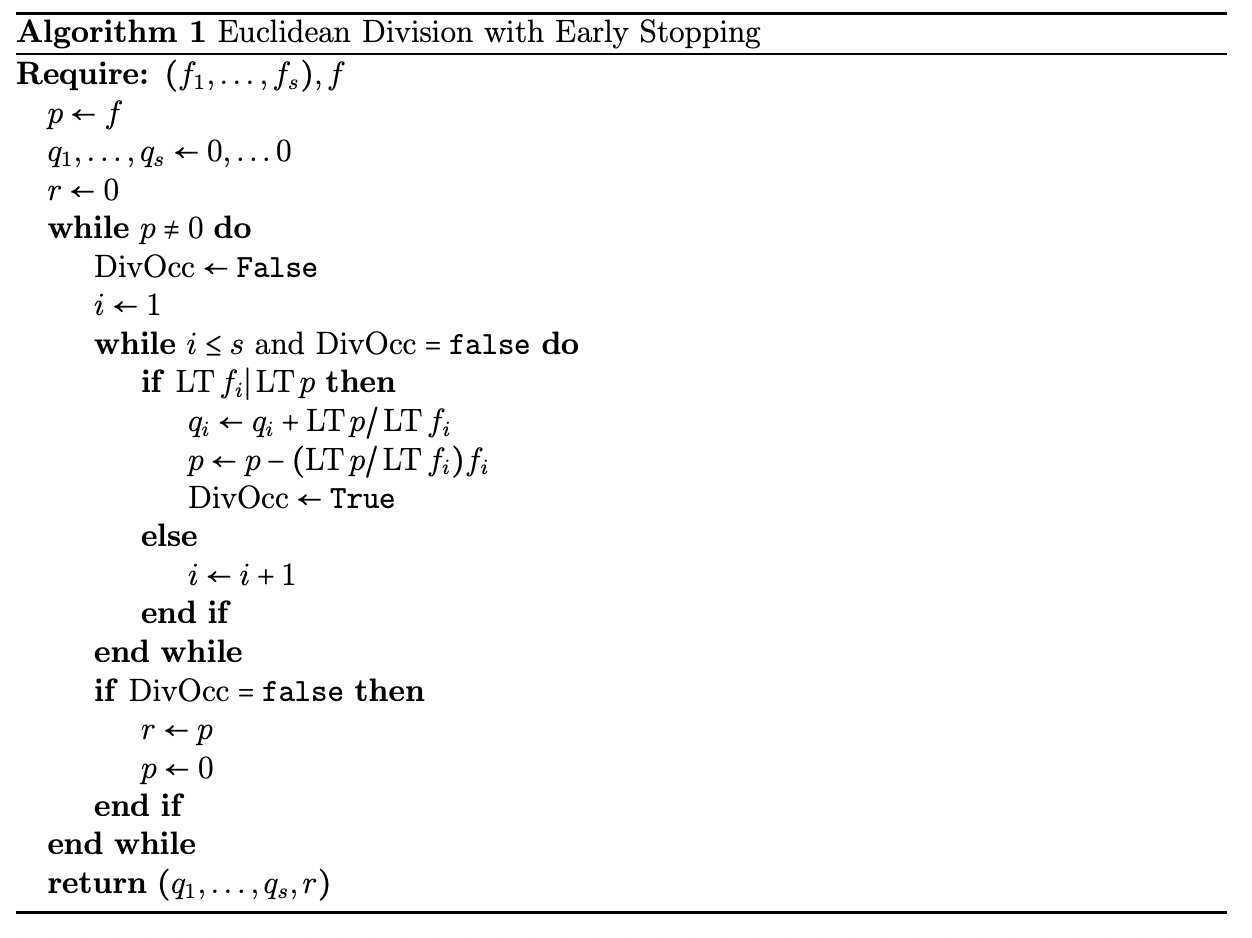
\includegraphics[width=\textwidth]{DivisionEarlyStopping.png}
		\end{figure}
	\end{frame}

\begin{frame}
	\frametitle{Buchberger with early stopping}
	\begin{figure}
		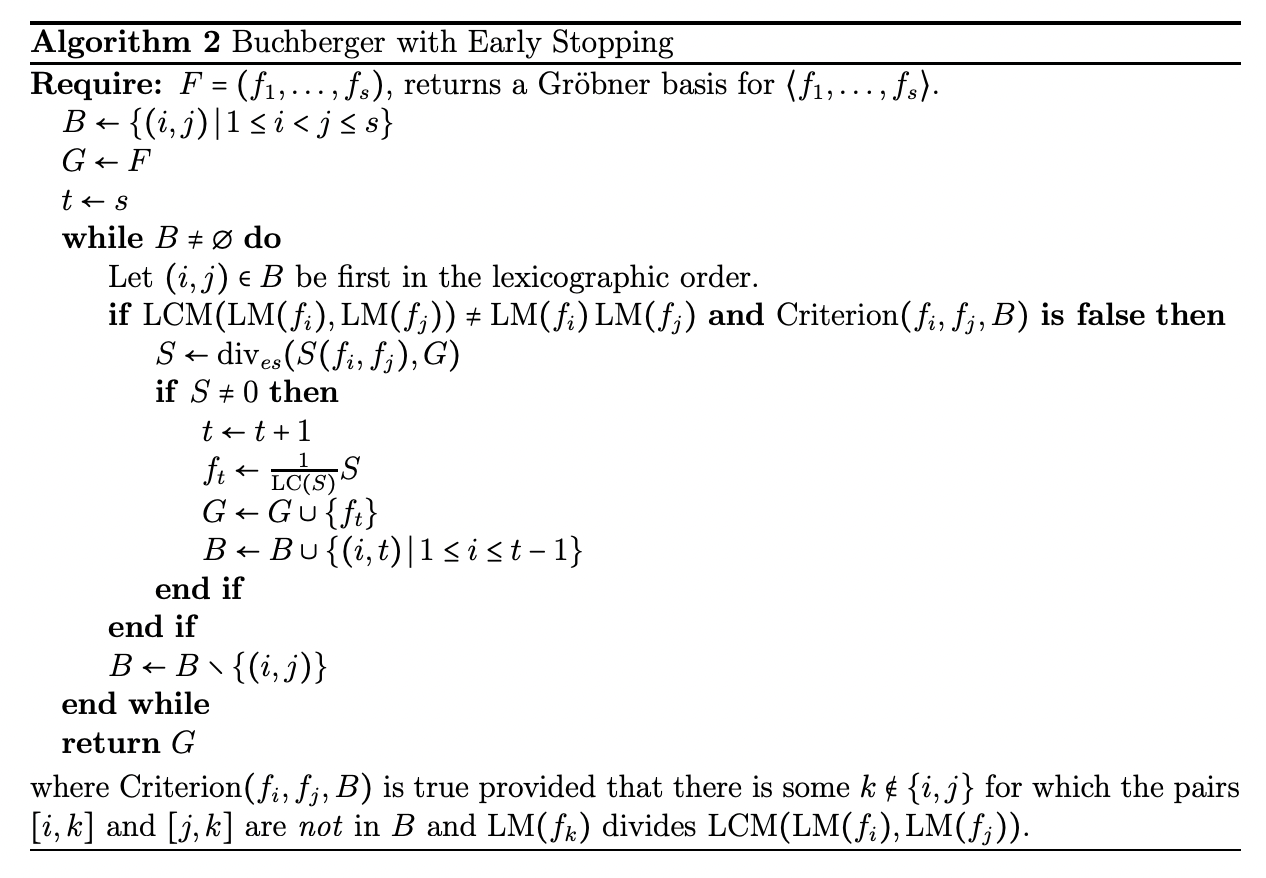
\includegraphics[width=\textwidth]{BuchbergerEarlyStopping.png}
		\end{figure}
	\end{frame}

\begin{frame}
	\frametitle{Elimination Theory}
	Let $\bold{X} = \{X_1,\ldots,X_n\}$ and $\bold{Y} = \{Y_1,\ldots,Y_m\}$ be variables. We suppose given an ideal $I \subseteq k[\bold{X}, \bold{Y}]$ and we are interested to know the equations between the $\bold{X}$-variables that are implied by the equations in $I$. We call this set of equations the elimination ideal:
	
	\begin{defn} The \emph{elimination ideal} of $I$ is the ideal $I \cap k[\bold{X}]$ in $k[\bold{X}]$.
	\end{defn}
	
	\begin{thm}[The Elimination Theorem]\label{thm:elimination} Let $I \subseteq k[\bold{X}, \bold{Y}]$ be an ideal and $G$ a Gröbner basis of $I$ with respect to a lexicographic order where $X_i < Y_j$ for all $1 \le i \le n, 1 \le j \le m$. Then $G \cap k[\bold{X}]$ is a Gröbner basis for $I \cap k[\bold{X}]$.
	\end{thm}
\end{frame}


\begin{frame}
	\frametitle{A graphical presentation}
	Fix a polynomial ring $k[X_1,\ldots,X_n]$, let $<$ be a total order on the set $\{X_1,\ldots,X_n\}$ and take the lexicographic monomial order determined by $<$. Let $\sigma$ be the permutation uniquely defined by
	\[
	X_{\sigma^{-1} 1} < X_{\sigma^{-1} 2} < \cdots < X_{\sigma^{-1} n}\,.
	\]
	The position of $X_i$ in this sequence is $\sigma(i)$. We view $\sigma$ as assigning a \emph{height} to variables:
	
	\begin{defn} The \emph{realisation} of $<$ is the oriented graph $\mathscr{R}_<$ with vertices
		\begin{equation}\label{eq:vertices_realisation}
			\big\{(i, \sigma i) \mid 1 \le i \le n \big\} \subseteq \mathbb{R}^2
		\end{equation}
		with an edge between $(i, \sigma i), (i+1, \sigma(i+1))$ for $i < n$, and $(i, \sigma i)$ decorated with $X_i$. The orientation of the edge is from $(i, \sigma i)$ to $(j, \sigma j)$ if $X_i < X_j$.
	\end{defn}
	\end{frame}

\begin{frame}
	\begin{defn} A \emph{$<$-graph} is an oriented graph on the vertex set \eqref{eq:vertices_realisation} with the property that if there is an edge from a vertex $(i, \sigma i)$ decorated with $X_i$ to a vertex decorated with $X_j$ then $X_i < X_j$.
	\end{defn}
	
	\begin{defn} A $<$-graph is \emph{linear} if every vertex has valence at most two.
	\end{defn}
	
	\begin{example}\label{example_allowedgraph_test} Let $X_1, \ldots, X_6$ be ordered by $X_5 < X_1 < X_6 < X_3 < X_2 < X_4$. Then $\mathscr{R}_<$ is
		\begin{equation}\label{eq:realisation_1}
			\adjustbox{scale=0.75}{\begin{tikzcd}[row sep = small, column sep = small, ampersand replacement=\&]
				\& \& \& X_4 \\
				\& X_2 \\
				\& \& X_3\\
				\& \& \& \& \& X_6 \\
				X_1\\
				\& \& \& \& X_5\\
				\arrow[from=5-1, to=2-2]
				\arrow[from=3-3, to=2-2]
				\arrow[from=3-3, to=1-4]
				\arrow[from=6-5, to=1-4]
				\arrow[from=6-5, to=4-6]
			\end{tikzcd}}
		\end{equation}
	\end{example}
	\end{frame}

\begin{frame}
	We simply write \emph{graph} instead of $<$-graph.
	
	\begin{defn} A \emph{roof} in a graph $\mathscr{S}$ is an ordered pair $(e,e')$ of edges $e: X_i \lto X_l, e': X_k \lto X_l$ with the same endpoint $X_l$ and $X_i < X_k$. We call $X_l$ the \emph{tip} of the roof.
	\end{defn}
	
	\begin{defn}\label{defn:gen_set_allowed} Given a graph $\mathscr{S}$ we define
		\[
		G_{\mathscr{S}} = \big\{ X_j - X_i \mid e: X_i \lto X_j \text{ is an edge in } \mathscr{S} \big\}\,.
		\]
	\end{defn}
	\end{frame}

\begin{frame}
	\frametitle{Standard monomial order}
	Let $\pi$ be a proof net with single conclusion $A$. Let
	\begin{equation}\label{eq:persistent_paths0}
		\mathscr{P}_1,\ldots,\mathscr{P}_m
	\end{equation}
	be the persistent paths of $\pi$ ordered so that if $U_i$ is the last unoriented atom in $\mathscr{P}_i$ then $U_1, \ldots, U_m$ is the order that these atoms appear in $A$. Let us name the variables $X_i$ so that \eqref{eq:persistent_paths0} is $X_1, \ldots, X_n$ and $P_\pi = k[X_1,\ldots,X_n]$.
	
	\begin{defn}\label{defn:monomial_order0} We write $U <_0 V$ if $U$ is before $V$ in \eqref{eq:persistent_paths0}. The monomial order $<_0$ on $P_\pi$ is the lexicographic order determined by $<_0$ on the variables.
	\end{defn}

\begin{defn}\label{defn:s_0} Let $\mathscr{S}_0$ be the oriented graph with vertex set $U_\pi$ where two variables $U, V \in U_\pi$ are connected by an edge $e: U \lto V$ if $U \sim V$ and $U <_0 V$.
\end{defn}
	\end{frame}

\begin{frame}
	\frametitle{Monomial order of a reduction sequence}
	$\Gamma: \pi \lto \pi'$ is a reduction sequence between proof nets with single conclusion $A$. Let $\mathscr{Q}_i$ be the subsequence of $\mathscr{P}_i$ consisting just of those unoriented atoms in $\pi'$ (those in the image of $T_\Gamma$). Let $\mathscr{P}_i \setminus \mathscr{Q}_i$ denote the complement of the subsequence $\mathscr{Q}_i$. Then
	\begin{equation}\label{eq:order_gamma}
		\mathscr{Q}_1, \ldots, \mathscr{Q}_m, \mathscr{P}_1 \setminus \mathscr{Q}_1,\ldots,\mathscr{P}_m \setminus \mathscr{Q}_m
	\end{equation}
	is the set of unoriented atoms of $\pi$ arranged in an order that depends on the reduction $\Gamma$. Note that $\mathscr{P}_i \setminus \mathscr{Q}_i$ are the variables in $\mathscr{P}_i$ eliminated during the reduction sequence.
	
	\begin{defn}\label{defn:monomial_order} We write $U <_\Gamma V$ if $U$ is before $V$ in \eqref{eq:order_gamma}, reading from left to right. The monomial order $<_\Gamma$ on $P_\pi$ is the lexicographic order determined by $<_\Gamma$ on the variables.
	\end{defn}
	\end{frame}

\begin{frame}
	\begin{defn}\label{defn:sequence_gpi0} We denote by $G^{(0)}_\pi$ the ordered set of polynomials $G_{\mathscr{S}_0}$
		\begin{equation}
			G^{(0)}_\pi = \big\{ V - U \mid e: U \lto V \text{ is an edge in } \mathscr{S}_0 \big\}\,.
		\end{equation}
	\end{defn}
\begin{defn}\label{defn:s_gamma} Let $\mathscr{S}_\Gamma$ be the oriented graph with vertex set $U_\pi$, where two variables $U, V \in U_\pi$ are connected by an edge $e: U \lto V$ if $U \sim V$ and $U <_\Gamma V$.
\end{defn}
\begin{defn} Given a sequence $F = (f_1,\ldots,f_s)$ of polynomials and a monomial order $<$ on $k[X_1,\ldots,X_n]$ we denote by $\mathbb{B}_{es}(F, <)$ the output of the Buchberger Algorithm with early stopping.
\end{defn}
\begin{thm}\label{thm:elimination_ours}
	There is an equality of sets
	\begin{equation}\label{eq:thm_elimination}
		G_{\pi'}^{(0)} = \mathbb{B}_{es}(G_{\pi}^{(\Gamma)}, <_\Gamma) \cap P_{\pi'}\,.
	\end{equation}
\end{thm}
	\end{frame}

\begin{frame}
	\frametitle{Falling Roofs}
	\Wider[4em]{
		\begin{defn} A roof $(e,e')$ precedes a roof $(d, d')$ if $e < d$ or $e = d$ and $e' < d'$.
		\end{defn}
	\begin{figure}
		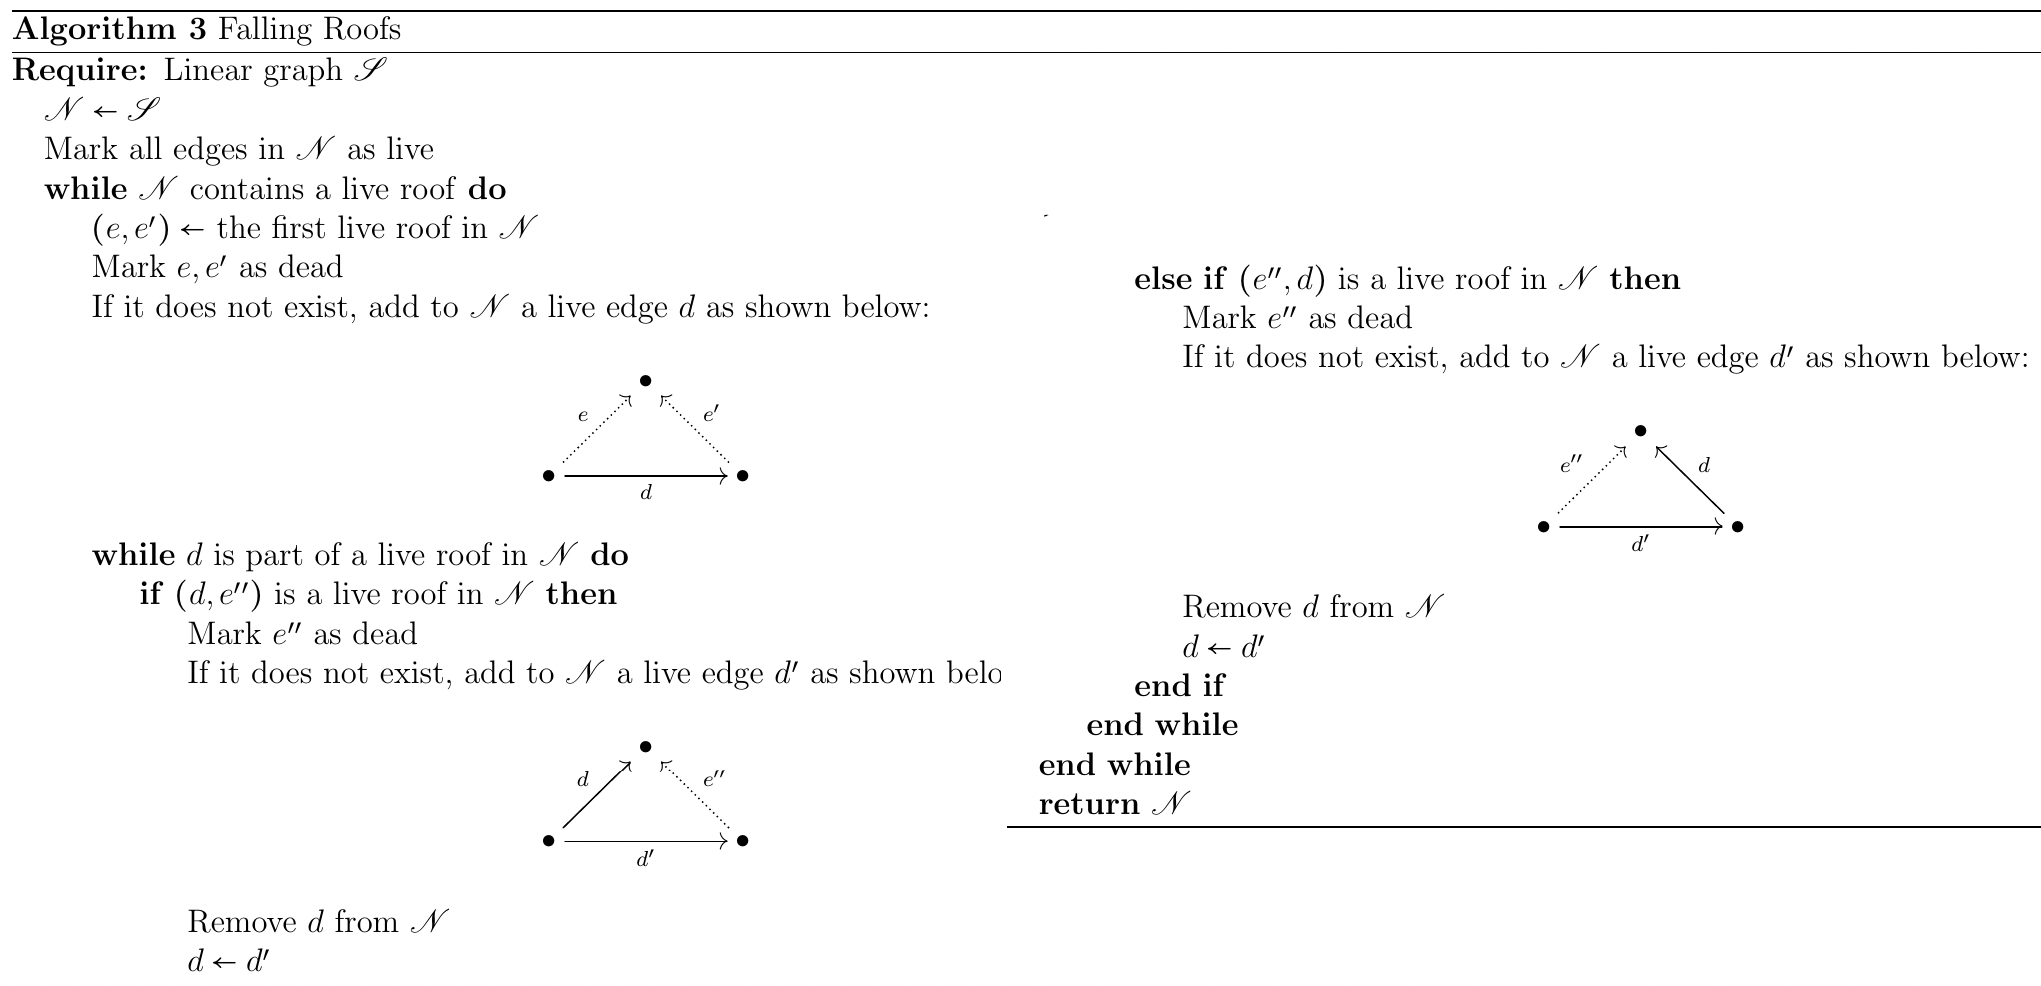
\includegraphics[width=\textwidth]{FallingRoofsOne.png}
		\end{figure}}
	\end{frame}

\begin{frame}
	\frametitle{Example}
	\begin{figure}
		\begin{center}
			\adjustbox{scale=0.55}{\begin{tabular}{ c c }
				\begin{tikzcd}[row sep = small, column sep = small, ampersand replacement=\&]
					\& \& \& X_4 \\
					\& X_2 \\
					\& \& X_3\\
					\& \& \& \& \& X_6 \\
					X_1\\
					\& \& \& \& X_5\\
					\arrow[from=5-1, to=2-2]
					\arrow[from=3-3, to=2-2]
					\arrow[from=3-3, to=1-4]
					\arrow[from=6-5, to=1-4]
					\arrow[from=6-5, to=4-6]
				\end{tikzcd}
				&
				\begin{tikzcd}[row sep = small, column sep = small, ampersand replacement=\&]
					\& \& \& X_4 \\
					\& X_2 \\
					\& \& X_3\\
					\& \& \& \& \& X_6 \\
					X_1\\
					\& \& \& \& X_5\\
					\arrow[dotted, from=5-1, to=2-2]
					\arrow[dotted, from=3-3, to=2-2]
					\arrow[from=5-1, to=3-3]
					\arrow[from=3-3, to=1-4]
					\arrow[from=6-5, to=1-4]
					\arrow[from=6-5, to=4-6]
				\end{tikzcd}
				\\
				\begin{tikzcd}[row sep = small, column sep = small, ampersand replacement=\&]
					\& \& \& X_4 \\
					\& X_2 \\
					\& \& X_3\\
					\& \& \& \& \& X_6 \\
					X_1\\
					\& \& \& \& X_5\\
					\arrow[dotted, from=5-1, to=2-2]
					\arrow[dotted, from=3-3, to=2-2]
					\arrow[from=5-1, to=3-3]
					\arrow[dotted, from=3-3, to=1-4]
					\arrow[dotted, from=6-5, to=1-4]
					\arrow[from=6-5,to=3-3]
					\arrow[from=6-5, to=4-6]
				\end{tikzcd}
				&
				\begin{tikzcd}[row sep = small, column sep = small, ampersand replacement=\&]
					\& \& \& X_4 \\
					\& X_2 \\
					\& \& X_3\\
					\& \& \& \& \& X_6 \\
					X_1\\
					\& \& \& \& X_5\\
					\arrow[dotted, from=5-1, to=2-2]
					\arrow[dotted, from=3-3, to=2-2]
					\arrow[dotted, from=5-1, to=3-3]
					\arrow[dotted, from=3-3, to=1-4]
					\arrow[dotted, from=6-5, to=1-4]
					\arrow[from=6-5,to=5-1]
					\arrow[from=6-5, to=4-6]
				\end{tikzcd}
			\end{tabular}}
		\end{center}
		\caption{The falling roofs algorithm applied to the graph of Example \ref{example_allowedgraph_test}, reading from left to right and top to bottom.}
		\label{figure:falling_roofs}
	\end{figure}
	\end{frame}

\begin{frame}
	What about Buchberger \emph{without} early stopping?
	\end{frame}

\begin{frame}
		Let $\pi$ denote the following proof net.
		% https://q.uiver.app/?q=WzAsMTMsWzEsMCwiXFxheCJdLFswLDEsIlhfMSJdLFswLDIsIlxcb3BlcmF0b3JuYW1le2N9Il0sWzIsMSwiWV8xIl0sWzMsMiwiXFxjdXQiXSxbNCwxLCJZXzIiXSxbNSwwLCJcXGF4Il0sWzYsMSwiWV8zIl0sWzcsMiwiXFxjdXQiXSxbOCwxLCJZXzQiXSxbMTAsMSwiWF8yIl0sWzksMCwiXFxheCJdLFsxMCwyLCJcXG9wZXJhdG9ybmFtZXtjfSJdLFswLDEsIiIsMCx7ImN1cnZlIjoyLCJzdHlsZSI6eyJoZWFkIjp7Im5hbWUiOiJub25lIn19fV0sWzEsMl0sWzAsMywiIiwyLHsiY3VydmUiOi0yLCJzdHlsZSI6eyJoZWFkIjp7Im5hbWUiOiJub25lIn19fV0sWzMsNCwiIiwyLHsiY3VydmUiOjJ9XSxbNSw0LCIiLDAseyJjdXJ2ZSI6LTJ9XSxbNiw1LCIiLDAseyJjdXJ2ZSI6Miwic3R5bGUiOnsiaGVhZCI6eyJuYW1lIjoibm9uZSJ9fX1dLFs2LDcsIiIsMix7ImN1cnZlIjotMiwic3R5bGUiOnsiaGVhZCI6eyJuYW1lIjoibm9uZSJ9fX1dLFsxMSw5LCIiLDAseyJjdXJ2ZSI6Miwic3R5bGUiOnsiaGVhZCI6eyJuYW1lIjoibm9uZSJ9fX1dLFsxMSwxMCwiIiwyLHsiY3VydmUiOi0yLCJzdHlsZSI6eyJoZWFkIjp7Im5hbWUiOiJub25lIn19fV0sWzEwLDEyXSxbOSw4LCIiLDAseyJjdXJ2ZSI6LTJ9XSxbNyw4LCIiLDIseyJjdXJ2ZSI6Mn1dXQ==
		\[\adjustbox{scale=0.7}{\begin{tikzcd}[column sep = small, row sep = small, ampersand replacement=\&]
			\& \ax \&\&\&\& \ax \&\&\&\& \ax \\
			{X_1} \&\& {Y_1} \&\& {Y_2} \&\& {Y_3} \&\& {Y_4} \&\& {X_2} \\
			{\operatorname{c}} \&\&\& \cut \&\&\&\& \cut \&\&\& {\operatorname{c}}
			\arrow[curve={height=12pt}, no head, from=1-2, to=2-1]
			\arrow[from=2-1, to=3-1]
			\arrow[curve={height=-12pt}, no head, from=1-2, to=2-3]
			\arrow[curve={height=12pt}, from=2-3, to=3-4]
			\arrow[curve={height=-12pt}, from=2-5, to=3-4]
			\arrow[curve={height=12pt}, no head, from=1-6, to=2-5]
			\arrow[curve={height=-12pt}, no head, from=1-6, to=2-7]
			\arrow[curve={height=12pt}, no head, from=1-10, to=2-9]
			\arrow[curve={height=-12pt}, no head, from=1-10, to=2-11]
			\arrow[from=2-11, to=3-11]
			\arrow[curve={height=-12pt}, from=2-9, to=3-8]
			\arrow[curve={height=12pt}, from=2-7, to=3-8]
		\end{tikzcd}}\]
		$\pi$ reduces to $\pi'$:
		% https://q.uiver.app/?q=WzAsNSxbMSwwLCJcXGF4Il0sWzAsMSwiWF8xIl0sWzIsMSwiWF8yIl0sWzIsMiwiXFxvcGVyYXRvcm5hbWV7Y30iXSxbMCwyLCJcXG9wZXJhdG9ybmFtZXtjfSJdLFswLDEsIiIsMCx7ImN1cnZlIjoyLCJzdHlsZSI6eyJoZWFkIjp7Im5hbWUiOiJub25lIn19fV0sWzAsMiwiIiwyLHsiY3VydmUiOi0yLCJzdHlsZSI6eyJoZWFkIjp7Im5hbWUiOiJub25lIn19fV0sWzEsNF0sWzIsM11d
		\[\adjustbox{scale=0.7}{\begin{tikzcd}[column sep = small, row sep = small, ampersand replacement=\&]
			\& \ax \\
			{X_1} \&\& {X_2} \\
			{\operatorname{c}} \&\& {\operatorname{c}}
			\arrow[curve={height=12pt}, no head, from=1-2, to=2-1]
			\arrow[curve={height=-12pt}, no head, from=1-2, to=2-3]
			\arrow[from=2-1, to=3-1]
			\arrow[from=2-3, to=3-3]
		\end{tikzcd}}\]
		We now consider the sets of generators of the defining ideals of $\pi$ and $\pi'$.
		\begin{equation*}
			G_\pi := \lbrace X_1 - Y_1, Y_1 - Y_2, Y_2 - Y_3, Y_3 - Y_4, Y_4 - X_2\rbrace,\quad G_{\pi'} := \lbrace X_1 - X_2 \rbrace
		\end{equation*}
		\begin{equation*}\label{eq:ordering}
			Y_1 > Y_2 > Y_3 > Y_4 > X_1 > X_2
		\end{equation*}
	\end{frame}

\begin{frame}
	\frametitle{There \emph{is} something to do}
	\[\adjustbox{scale=0.7}{\begin{tikzcd}[column sep = small, row sep = small, ampersand replacement=\&]
			\& \ax \&\&\&\& \ax \&\&\&\& \ax \\
			{X_1} \&\& {Y_1} \&\& {Y_2} \&\& {Y_3} \&\& {Y_4} \&\& {X_2} \\
			{\operatorname{c}} \&\&\& \cut \&\&\&\& \cut \&\&\& {\operatorname{c}}
			\arrow[curve={height=12pt}, no head, from=1-2, to=2-1]
			\arrow[from=2-1, to=3-1]
			\arrow[curve={height=-12pt}, no head, from=1-2, to=2-3]
			\arrow[curve={height=12pt}, from=2-3, to=3-4]
			\arrow[curve={height=-12pt}, from=2-5, to=3-4]
			\arrow[curve={height=12pt}, no head, from=1-6, to=2-5]
			\arrow[curve={height=-12pt}, no head, from=1-6, to=2-7]
			\arrow[curve={height=12pt}, no head, from=1-10, to=2-9]
			\arrow[curve={height=-12pt}, no head, from=1-10, to=2-11]
			\arrow[from=2-11, to=3-11]
			\arrow[curve={height=-12pt}, from=2-9, to=3-8]
			\arrow[curve={height=12pt}, from=2-7, to=3-8]
	\end{tikzcd}}\]
	\begin{equation*}
		G_\pi = \lbrace \textcolor{blue}{f_1= } X_1 - Y_1, \textcolor{blue}{f_2= }Y_1 - Y_2, \textcolor{blue}{f_3= }Y_2 - Y_3, \textcolor{blue}{f_4= }Y_3 - Y_4, \textcolor{blue}{f_5= }Y_4 - X_2\rbrace
	\end{equation*}
\begin{equation*}
	Y_1 > Y_2 > Y_3 > Y_4 > X_1 > X_2
\end{equation*}
	The leading terms of $f_1,...,f_5$ respectively are $-Y_1, Y_1, Y_2, Y_3, Y_4$ and the leading term of $f_1 + \hdots + f_5$ is $X_1$. Hence:
	\begin{equation*}
		X_1 \in \operatorname{LT}\langle G_\pi \rangle ,\qquad  X_1 \not\in\langle \operatorname{LT}G_\pi \rangle
		\end{equation*}
	Thus, $G_\pi$ is \emph{not} Gr\"{o}bner basis.
	\end{frame}

\begin{frame}
	We now calculate the $10$ $S$-polynomials which arise from $G_\pi$.
	\begin{equation*}\adjustbox{scale=0.7}{\begin{tikzcd}[ampersand replacement=\&, row sep = tiny]
				S(f_1,f_2) = Y_2 - X_1 \& S(f_1, f_3) = Y_1Y_3 - Y_2 X_1 \& S(f_1,f_4) = Y_1Y_4 - X_1X_3\\
				S(f_1,f_5) = Y_1X_2 - X_1Y_4 \& S(f_2,f_3) = Y_1Y_3 - Y_2^2 \& S(f_2,f_4) = Y_1Y_4 - Y_2Y_3\\
				S(f_2,f_5) = Y_1X_2 - Y_2Y_4 \& S(f_3,f_4) = Y_2Y_4 - Y_2^2 \& S(f_3,f_5) = Y_2X_2 - Y_3Y_4\\
				S(f_4,f_5) = Y_3X_2 - Y_4^2\end{tikzcd}}
	\end{equation*}
	For each $i > j$, $i,j \in \lbrace 1,...,5\rbrace$ we now divide $S(f_i,f_j)$ by $G$. In fact, this always gives a remainder zero except for the particular case when $(i,j) = (1,2)$, which we show on the next slide.
	\end{frame}

\begin{frame}
	\frametitle{Division}
	\[\adjustbox{scale=0.7}{\begin{tikzcd}[column sep = small, row sep = small, ampersand replacement=\&]
			\& \ax \&\&\&\& \ax \&\&\&\& \ax \\
			{X_1} \&\& {Y_1} \&\& {Y_2} \&\& {Y_3} \&\& {Y_4} \&\& {X_2} \\
			{\operatorname{c}} \&\&\& \cut \&\&\&\& \cut \&\&\& {\operatorname{c}}
			\arrow[curve={height=12pt}, no head, from=1-2, to=2-1]
			\arrow[from=2-1, to=3-1]
			\arrow[curve={height=-12pt}, no head, from=1-2, to=2-3]
			\arrow[curve={height=12pt}, from=2-3, to=3-4]
			\arrow[curve={height=-12pt}, from=2-5, to=3-4]
			\arrow[curve={height=12pt}, no head, from=1-6, to=2-5]
			\arrow[curve={height=-12pt}, no head, from=1-6, to=2-7]
			\arrow[curve={height=12pt}, no head, from=1-10, to=2-9]
			\arrow[curve={height=-12pt}, no head, from=1-10, to=2-11]
			\arrow[from=2-11, to=3-11]
			\arrow[curve={height=-12pt}, from=2-9, to=3-8]
			\arrow[curve={height=12pt}, from=2-7, to=3-8]
	\end{tikzcd}}\]
	\begin{equation*}
		G_\pi = \lbrace \textcolor{blue}{f_1= } X_1 - Y_1, \textcolor{blue}{f_2= }Y_1 - Y_2, \textcolor{blue}{f_3= }Y_2 - Y_3, \textcolor{blue}{f_4= }Y_3 - Y_4, \textcolor{blue}{f_5= }Y_4 - X_2\rbrace
	\end{equation*}
	\begin{equation*}
		\begin{array}{rll}
			& (0,0,1,1,1)\\
			G_\pi & \showdiv{Y_2 - X_1}\\
			%
			&\hspace{0.55em} Y_2 - Y_3\\
			\CMidRule[3.0ex][10.0ex]{2-2}
			&\hspace{0.55em} \hphantom{Y_2 +{}}  Y_3 - Y_4\\
			&\hspace{0.55em} \hphantom{Y_2 +{}}  Y_3 - X_1\\
			\CMidRule[7.0ex][5.0ex]{2-2}
			&\hspace{0.55em} \hphantom{Y_2 - Y_3 +{}} Y_4 - X_1\\
			&\hspace{0.55em}\hphantom{Y_2 - Y_3 +{}} Y_4 - X_2\\
			\CMidRule[11.0ex][0.0ex]{2-2}
			&\hspace{0.55em} \hphantom{Y_2 - Y_3 + Y_4 + {}} X_2 - X_1
		\end{array}
	\end{equation*}
\begin{equation*}
	\big(G_\pi \cup \lbrace X_2 - X_1 \rbrace\big) \cap k[X_1,X_2] = G_{\pi'}
	\end{equation*}
\end{frame}

\begin{frame}
	\frametitle{Summary}
	\begin{equation}\label{eq:proof_to_ideal}
		\pi \longmapsto (P_\pi, G_\pi, <_0)
	\end{equation}
There are many other monomial orders on $P_\pi$. With respect to some monomial orders $G_\pi$ will be ``stable'' in the sense that it is a Gröbner basis, while it will be ``unstable'' (not a Gröbner basis) with respect to others and running the Buchberger algorithm makes nontrivial changes.

\begin{figure}
	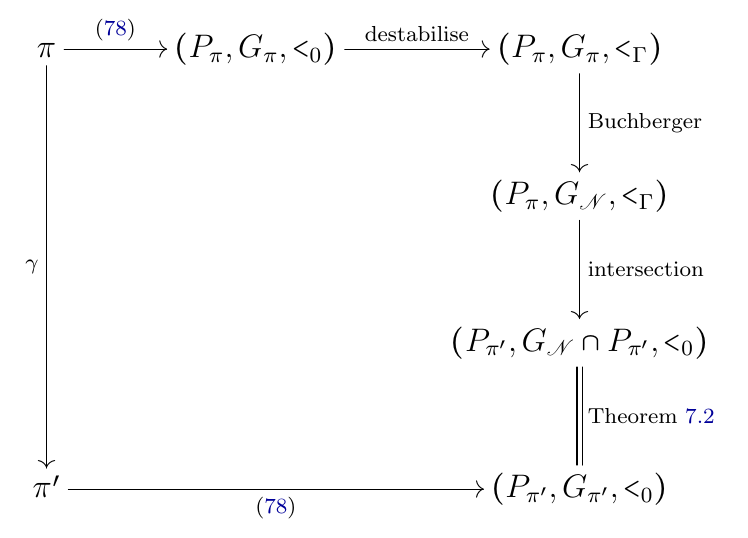
\includegraphics[width=0.65\textwidth]{ConclusionAlgPnt.png}
\end{figure}
	\end{frame}

\begin{frame}[allowframebreaks]
	\begin{thebibliography}{9}
		\bibitem{Boole} G.~Boole, \textsl{An Investigation into the Laws of Thought} (1854).
		\bibitem{Grobner} D. Cox, J. Little, D. O'Shea, \emph{Ideals, Varieties, and Algorithms} Fourth Edition, Springer (2015).
		
		\bibitem{girard_llogic}
		J.-Y.~Girard, \textsl{Linear Logic}, Theoretical Computer Science 50 (1), 1--102 (1987).
		
		\bibitem{Girard} J.-Y.~Girard, \emph{Multiplicatives}, Logic and Computer Science: New Trends and Applications. Rosenberg \& Sellier. pp. 11–34 (1987).
		
		\bibitem{towards_goi}
		J.-Y.~Girard, \textsl{Towards a geometry of interaction}, In J.~W.~Gray and A.~Scedrov, editors, Categories in Computer Science and Logic, volume 92 of Contemporary Mathematics, 69--108, AMS (1989).
		
		\bibitem{bs}
		J.-Y.~Girard, \textsl{The Blind Spot: lectures on logic}, European Mathematical Society, (2011).
		
		\bibitem{proofstypes}
		J.-Y.~Girard, Y.~Lafont, and P.~Taylor, \textsl{Proofs and Types}, Cambridge Tracts in Theoretical Computer Science 7 ,Cambridge University Press (1989).
		
		\bibitem{howard} W.~A.~Howard, \textsl{The formulae-as-types notion of construction}, in Seldin and Hindley \textsl{To H.B.Curry: essays on Combinatory logic, Lambda calculus and Formalism}, Academic press (1980).
		
		\bibitem{Laurent} O. Laurent, \emph{An Introduction to Proof Nets}, \url{http://perso.ens-lyon.fr/olivier.laurent/pn.pdf} (2013).
		
		\bibitem{murfet_ll}
		D.~Murfet, \textsl{Logic and Linear Algebra: An Introduction}, preprint \url{https://arxiv.org/abs/1407.2650v3} (2017).
		
		\bibitem{gmz} D.~Murfet and W.~Troiani, \textsl{{G}entzen-{M}ints-{Z}ucker duality}, preprint \url{https://arxiv.org/abs/2008.10131} (2020).
		
		\bibitem{Troiani} W. Troiani, \emph{Linear logic}, lecture notes \url{https://williamtroiani.github.io/MathNotes/LinearLogic.pdf} (2020).
		\end{thebibliography}
	\end{frame}
	
\end{document}